\documentclass[english,12pt,a4paper,pdftex,sci,utf8]{aaltothesis}
\usepackage{graphicx}
\usepackage{amsfonts,amssymb,amsbsy}

\usepackage{tabularx}
\usepackage{csquotes}
\usepackage{biblatex}
\usepackage{enumitem}
\usepackage{textgreek}
\usepackage{amsthm}
\usepackage{blkarray}
\usepackage{amsmath}
\usepackage{subcaption}

\addbibresource{bibliography.bib}

\theoremstyle{definition}
\newtheorem{definition}{Definition}
\usepackage{hyperref}
\PackageWarning{NYI}{Remember to edit this}
\hypersetup{pdfpagemode=UseNone, pdfstartview=FitH,
  colorlinks=true,urlcolor=red,linkcolor=blue,citecolor=black,
  pdftitle={Default Title, Modify},pdfauthor={Teemu Vartiainen},
  pdfkeywords={Modify keywords}}

% custom command for edit comments
\definecolor{nyitext}{rgb}{0.2, 0.2, 0.2}
\definecolor{nyibg}{rgb}{1.0, 1.0, 0.6}
\newcommand{\nyi}[1]{\noindent\colorbox{nyibg}{\textcolor{nyitext}{\emph{#1}}}}

%\PackageWarning{NYI}{#1}

%\setlength{\parskip}{0.5ex}
%\linespread{1.2}

\begin{document}
\department{Department of Computer Science}
\professorship{x}
\univdegree{MSc}
\author{Teemu Vartiainen}

%% Your thesis title comes here and again before a possible abstract in
%% Finnish or Swedish . If the title is very long and latex does an
%% unsatisfactory job of breaking the lines, you will have to force a
%% linebreak with the \\ control character. 
%% Do not hyphenate titles.
\thesistitle{Analyzing real-time and past events to discover processes and to detect anomalies}

\place{Espoo}

\date{x.x.2017}
\supervisor{Prof.\ Petri Vuorimaa}
\advisor{M.Sc.\ Tao Zhu}
\advisor{M.Sc.\ Rafael Forsbach Valle}

\uselogo{aaltoBlue}{?}

\makecoverpage

%%%%%%%%%%%%%%%%%%%%%%%%%%%%%%%%%%%%%%%%%%%%%%%%%%%%%%%%%%%%%%%%%%%%%%%%%%%%%%%%
%%% Meta stuff
%%%%%%%%%%%%%%%%%%%%%%%%%%%%%%%%%%%%%%%%%%%%%%%%%%%%%%%%%%%%%%%%%%%%%%%%%%%%%%%%
% 
%%%%%%%%%%%%%%%%%%%%%%%%%%%%%%%%%%%%%%%%%%%%%%%%%%%%%%%%%%%%%%%%%%%%%%%%%%%%%%%%
%%% Abstracts & etc
%%%%%%%%%%%%%%%%%%%%%%%%%%%%%%%%%%%%%%%%%%%%%%%%%%%%%%%%%%%%%%%%%%%%%%%%%%%%%%%%

\keywords{Process discovery, Machine learning, Event logs}

%% Abstract text
\begin{abstractpage}[english]
  Your abstract in English. Try to keep the abstract short; approximately 
  100 words should be enough. The abstract explains your research topic, 
  the methods you have used, and the results you obtained.  
  Your abstract in English. Try to keep the abstract short; approximately 
  100 words should be enough. The abstract explains your research topic, 
  the methods you have used, and the results you obtained.  

  Your abstract in English. Try to keep the abstract short; approximately 
  100 words should be enough. The abstract explains your research topic, 
  the methods you have used, and the results you obtained.  
  Your abstract in English. Try to keep the abstract short; approximately 
  100 words should be enough. The abstract explains your research topic, 
  the methods you have used, and the results you obtained.  
\end{abstractpage}

\newpage

%% Abstract in Finnish.

\thesistitle{Reaaliaikaisten ja menneiden prosessitapahtumien k\"aytt\"o prosessitutkinnassa ja poikkeavuuksien havainnassa}
\supervisor{Prof.\ Petri Vuorimaa}
\advisor{M.Sc.\ Tao Zhu}
\advisor{M.Sc.\ Rafael Forsbach Valle}
\department{Tietotekniikan laitos}
\professorship{x}
%% Avainsanat
\keywords{Prosessitutkinta, Koneoppiminen, Tapahtumalokit}
%% Tiivistelmän tekstiosa
\begin{abstractpage}[finnish]
  Tiivistelmässä on lyhyt selvitys (noin 100 sanaa)
  kirjoituksen tärkeimmästä sisällöstä: mitä ja miten on tutkittu,
  sekä mitä tuloksia on saatu. 
  Tiivistelmässä on lyhyt selvitys (noin 100 sanaa)
  kirjoituksen tärkeimmästä sisällöstä: mitä ja miten on tutkittu,
  sekä mitä tuloksia on saatu. 

  Tiivistelmässä on lyhyt selvitys (noin 100 sanaa)
  kirjoituksen tärkeimmästä sisällöstä: mitä ja miten on tutkittu,
  sekä mitä tuloksia on saatu. 
  Tiivistelmässä on lyhyt selvitys (noin 100 sanaa)
  kirjoituksen tärkeimmästä sisällöstä: mitä ja miten on tutkittu,
  sekä mitä tuloksia on saatu. 
  Tiivistelmässä on lyhyt selvitys (noin 100 sanaa)
  kirjoituksen tärkeimmästä sisällöstä: mitä ja miten on tutkittu,
  sekä mitä tuloksia on saatu. 
\end{abstractpage}

%% Preface
\mysection{Preface}

This thesis work was carried out at the Microsoft headquarters at the campus in Redmond, USA.
It has been written as the last part of my Master's degree.

I would like to thank the people at Microsoft for the opportunity.
Thank you Kristin and Britt at recruiting for figuring out the unusual circumstances for me.
Thank you Tao and Rafael for mentoring and guiding me during my work.
I would also like to thank the rest of the ICH Catalog Health team for dealing with my constant questions
and helping me feel like home in my team.

Great thanks to professor Petri Vuorimaa for being my supervisor and for helping me with the practicalities.

I would like to thank my friends for supporting me.
I would like to thank my girlfriend Kara for her unending support and understanding during this stressful time.
It is not an understatement that without you I would not be where I am today.
Thank you Max and David for your endless support and for proofreading.
Thank you Xane, Jorge, Cody, and other friends and birds for keeping me sane.

Lastly I would like to thank all my family for standing by me and dealing with my travels and schedules.

\vspace{5cm}
Espoo, y.y.2017

\vspace{5mm}
{\hfill Teemu T.\ Vartiainen \hspace{1cm}}

\newpage
\thesistableofcontents

\mysection{Symbols and Abbreviations placeholder}

\subsection*{Symbols}

\begin{tabular}{ll}
$\mathbb{B}(X)$  & a set of multi-sets over $X$ \\
$\emptyset$      & empty set \\
\end{tabular}

\subsection*{Operators}

\begin{tabular}{ll}
$a \in A$    & $a$ is a member of set $A$ \\
$A \cap B$   & intersection of sets $A$ and $B$ \\
\end{tabular}

\subsection*{Abbreviations}

\begin{tabular}{ll}
BDT         & boosted decision tree \\
BI          & business intelligence \\
MBI         & medium business intelligence \\
ML          & machine learning \\
MSE         & mean square error \\
PII         & personally identifiable information \\
SLA         & service level agreement \\
SQL         & structured query language \\
TP          & top percentile \\
\end{tabular}

%%%%%%%%%%%%%%%%%%%%%%%%%%%%%%%%%%%%%%%%%%%%%%%%%%%%%%%%%%%%%%%%%%%%%%%%%%%%%%%%

\cleardoublepage
\storeinipagenumber
\pagenumbering{arabic}
\setcounter{page}{1}

%%%%%%%%%%%%%%%%%%%%%%%%%%%%%%%%%%%%%%%%%%%%%%%%%%%%%%%%%%%%%%%%%%%%%%%%%%%%%%%%
%%%%%%%%%%%%%%%%%%%%%%%%%%%%%%%%%%%%%%%%%%%%%%%%%%%%%%%%%%%%%%%%%%%%%%%%%%%%%%%%
%%% Content starts here
%%%%%%%%%%%%%%%%%%%%%%%%%%%%%%%%%%%%%%%%%%%%%%%%%%%%%%%%%%%%%%%%%%%%%%%%%%%%%%%%
%%%%%%%%%%%%%%%%%%%%%%%%%%%%%%%%%%%%%%%%%%%%%%%%%%%%%%%%%%%%%%%%%%%%%%%%%%%%%%%%

% %%%%%%%%%%%%%%%%%%%%%%%%%%%%%%%%%%%%%%%%%%%%%%%%%%%%%%%%%%%%%%%%%%%%%%%%%%%%%%%%
%%% Introduction
%%%%%%%%%%%%%%%%%%%%%%%%%%%%%%%%%%%%%%%%%%%%%%%%%%%%%%%%%%%%%%%%%%%%%%%%%%%%%%%%

\section{Introduction}
\thispagestyle{empty}

\subsection{Motivation}
%       Importance of accurate real time data
Having diagnostics and real-time data is important in modern software operations.
Dashboards, visualizations, and interactive logging is becoming more and more important
in the quickly changing digital world. Often these solutions are labeled Business Intelligence.
Having an accurate sense of current system status and low response time to faults can provide an advantage
in business against competitors.

%       Importance of having both a big picture and detailed view of current processes
%         Information tailored to different people

In software operations, many stakeholders are interested in this information. 
These stakeholders come from different backgrounds with different kinds of expertise.
and can include, among others, developers, system administrators, project managers, and partner representatives.
This means that not all people interested in the information have the same level of technical ability to interpret, for example, raw system logs. 
Additionally, there may be issues of confidentiality, and it is often important to control who can see what data.

Furthermore, different people are interested in different granularities of information.
The engineers might want to see fine detail whereas higher level managers want aggregation and averages.
Thus, having customizable views for this data can be crucial,
since the users want to only see the information that helps them in their jobs.
%       Predicting future events to give information and schedule tasks
In addition to views of the present, a peek into the future can provide a major advantage.
Being able to predict what happens soon in the future helps with scheduling tasks and lets people react 
to events before they happen. With technologies like machine learning we can learn patterns in data and 
start estimating information beyond the present time.

%       Loosely coupling diagnostics from systems
%       Adapting to change in agile and quickly changing environment
Another aspect of software operations is that they are ever-changing: today's bleeding edge is tomorrow's obsolete. 
A tightly coupled diagnostics system becomes useless when the system or workflow changes significantly. 
Any analytics or visualization solution should be agnostic to what the system does in reality and what specific technologies it uses. 
This keeps the solution relevant for a long lifetime and enables it to be useful for different systems in different environments. 
To save costs and time the solution should adapt to change seamlessly without constant maintenance from the users or the system administrators. However, unintended changes should be detected and notified about.

%   not as easy as it seems
All these goals come together to form a challenge in modern software operations.
The systems being monitored are complex, distributed, and interconnected.
Providing business intelligence in real-time, showing different information to different people, and dynamically adapting to change are all difficult tasks on their own and trying to succeed in all of them is an even bigger challenge to solve.
The solution to this is a system that is able to succeed in these three aspects without human involvement.

\subsection{Microsoft}
%        store with tons of products and parallel workflows ongoing continuously
At a multinational company as large as Microsoft the scale of information is staggering.
Distributed systems process data and generate log entries concurrently in the numbers of terabytes.
No single person can monitor all the logs from even a single system without the help of automated
graphs, alerts, and notifications.  

% relate this into the store
One of these systems is the Microsoft Windows store. The store contains hundreds of thousands of products
such as apps and games. Publishers such as software companies and individual developers submit thousands of 
products to the store each day. Before the products reach the public retail store, however, they need to be processed
through a pipeline of multiple steps. These steps can data collection, validating the package integrity, and
other automated and manual checks to make sure the product should be allowed in the store,
and that the store systems have all the information they need to function.
Each product submission produces log entries that document these steps.

%        many different users need different kinds of information
%        third party developers and customers want to know what is going on
These system log entries are collected and stored as they happen. 
Different stakeholders from software developers and engineers to third-party publishers and retail users 
may benefit from this data. However, the needs for each of them are
different with regards to detail and types of information.
The engineers often need very detailed information from all the processes and parts of the system to debug an issue in real-time,
while a third party submitting a product may only be concerned with the big picture of whether their 
product is available in the retail store or not.

Furthermore, concerns of privacy and confidentiality further complicate this issue.
For example, the detailed information the engineers need is often confidential to Microsoft or its partners.
The product publishers need access to the statistics of their own products, but should not see data that belongs to other publishers.
This information is business-critical when Microsoft is dealing with high profile publishers such as high-profile game companies.

%            we need to be able to answer and provide a good service
%        detecting failures is essential to keep up SLAs and good experience
%            automation, prioritization, customization
When running the store, Microsoft is providing a service to retail customers and product publishers.
To provide good service, the goal is to be transparent enough that the maintenance and operation of the store do not hinder the business of the customers. 
Providing accurate information and time estimations to the publishers
not only helps Microsoft internally, but also helps the publishers' business.
In addition, Microsoft must adhere to contracts such as
service level agreements (SLA) which determine, among other metrics, 
maximum response times and lengths for various processes.
For example, there is an SLA for how long a product submission can take from the beginning to when it is available in the store.

Like in any complex system, sometimes things go wrong.
When an issue arises, engineers and managers need to have tools to investigate what is happening. 
The store pipeline consists of multiple separate systems and workflows processing the incoming products.
Detecting faults as they happen is crucial for the people responsible for maintaining the system.
If such a workflow does not have detailed monitoring functionality, 
finding the details to investigate an issue proves to be challenging.
This kind of workflow is, in essence, a black box system, since there is no information for an outside observer
about the internal state;
they are only able to see whether the workflow is running or has been completed.
In addition, the duration of these workflows can vary greatly from seconds to hours to days.

This is where an intelligent logging, visualization, and notification tool is needed. 
A solution that provides both the big picture and the details will help investigate issues faster and
provide good service to third party publishers and customers.
When the people responsible have all the right information they are able to assess the severity of anomalies and prioritize their time.
This allows Microsoft to provide a good service.

\subsection{Research goals}
%		Questions and elaboration
%       Scope and main concepts of research
In this thesis I investigated methods for monitoring and visualizing the product submission workflows in the Microsoft Windows store.
These workflows are triggered based on real world events, often by developers submitting applications and games to the store.
I investigated ways of analyzing these workflows in real time and providing useful information to different users with different needs. 

I carried out research and development at Microsoft to answer the following research questions:

\begin{enumerate}[label=RQ\arabic*]
    \item How can a real-time event log from multiple sources and multiple concurrent workflows be dynamically transformed into a model that describes the process? 
    \item How can the model and past log data be used to predict future events and their times?
    \item How can the predictions be used to detect anomalies in new events (or lack thereof)?
\end{enumerate}

For the first question (RQ1), the goal was to have an unsupervised monitoring system 
that uses the current and past logs to automatically determine all the actors, 
workflows, and steps related to the product submissions.
The store pipeline is constantly being developed further to be faster and to include more functionality.
The system should require as little maintenance as possible, instead retraining itself automatically and often to adapt to change.
In addition, the project should include as little hardcoded configuration as possible.

The second goal for the project was the capability to estimate future events within the system (RQ2). 
Many stakeholders are interested in the pipeline completion times, so they can schedule their tasks accordingly.
Comparisons between the estimations and the realized event times should be used to notify people about any anomalies, faults, or delays in the pipeline that are relevant to them (RQ3).

A further goal for the project developed in this thesis was that it should not be tightly coupled to the 
specific submission workflows in the store. The solution should not depend on the specific activities so
it requires less maintenance and can be reused in other systems.

\subsection{Structure of the Thesis}
%   d. Structure of thesis
This thesis is divided in six sections. In the first section I have introduced the motivation for this research first by looking at the industry as a whole and then from Microsoft's standpoint.
I have also laid out the research questions I will answer in this thesis.
Section 2 describes the background knowledge required to understand the methods used in this thesis.
I introduce process mining and the theory behind it. I will also briefly introduce the concept of machine learning.

Section 3 describes the problem being solved in this thesis. I will introduce the context and the needed understanding about the store system relevant to this thesis. I will also describe the requirements engineering work I did to find the requirements for the project.
In section 4 I describe the project starting point and its time line.
I will describe and all the materials and the data used for the project.

Section 5 outlines the methods used to solve the research questions.
In the section I describe how I applied to theory in the project.
I also describe the user interface created during the project.
Finally in section 6 I describe the results of the whole thesis project and evaluate them.

% %%%%%%%%%%%%%%%%%%%%%%%%%%%%%%%%%%%%%%%%%%%%%%%%%%%%%%%%%%%%%%%%%%%%%%%%%%%%%%%%
%%% Background
%%%%%%%%%%%%%%%%%%%%%%%%%%%%%%%%%%%%%%%%%%%%%%%%%%%%%%%%%%%%%%%%%%%%%%%%%%%%%%%%

%% In a thesis, every section starts a new page, hence \clearpage
\clearpage
\section{Background and related work}
\label{sec:background}

\subsection{Process mining}

Process mining starts from the concept of an \emph{event log}.
An event log is a collection of recorded data for an information system.
Activities executed in the system leave records which are stored in the event log.
\emph{Process mining} describes methods of using the event log data to extract useful information.
The information can be used to discover processes without prior knowledge, to find bottlenecks and inefficiencies, to detect and understand anomalies, and to support redesign actions \cite{van2015extracting}.
In this thesis I look at \emph{process discovery}, which means finding the underlying process model
by reading the event log.
In process discovery the model should be generated without any a-priori information, meaning that the algorithm should be unsupervised \cite{van2013discovering}.
The process model can be expressed as a directed graph or a \emph{Petri net}.
These models can be used for business intelligence (BI) solutions, or they can be compared to the real life
known models to check conformance \cite{van2013discovering}.


Discovering strictly sequential processes from event logs is straightforward. However, modern systems are increasingly concurrent which complicates the issue. 
Parallel systems generate events in a undetermined order based on how the processes are interleaved. 
When the events are logged the order is realized resulting in a totally ordered sequential log \cite{van2004workflow}. 
The challenge is having to discover and construct the parallelism from the event log.
Furthermore, the event log may be \emph{incomplete}, which means not all possible behaviour is present in the logs \cite{van2013discovering}.
Additionally, the event logs can be \emph{noisy} and contain random infrequent behaviour \cite{van2013discovering}.
It may be undesirable to present the infrequent behaviour in the models.
These characteristics give the task of process discovery challenging trade-offs.

\subsubsection{Event logs and traces}

\label{sec:eventtheory}

\begin{definition}
Let $A$ be the set of all \emph{activities}. 
$\sigma \in A^*$ is a workflow trace describing a \emph{sequence of events}.
The event log $L \in \mathbb{B}(A^*)$ is a \emph{multi-set} of \emph{traces}.
\end{definition}

A process consists of a set of distinct \emph{activities}.
An activity is a well-defined step belonging to the process.
Each event in the event log refers to such an activity.
The event may also hold additional information about the process.
A workflow \emph{trace} contains a sequence of events documenting a single execution of the process (a \emph{process instance}).
This kind of single process execution is called a \emph{case} (later in this thesis also: \emph{submission}).
The event log can be seen as a \emph{multi-set} of \emph{traces}. 
A multi-set (a \emph{bag}) is a set that allows multiple instances of the set's elements. \cite{van2015extracting}

In this thesis it is assumed that any concurrent execution of events can be recorded into
an ordered and sequential event log. 
The concurrent execution generates randomly ordered sequences.
The parallelisms can be discovered by observing the different traces and their frequencies.
For example, for a process consisting of activities $a,b,c,d,e \in A$, one trace could be 
$\langle a,b,c,d,e \rangle$ and another $\langle a,c,d,b,e \rangle$ \nyi{see figure}.
These different traces could be found in the event log a number of times, some more frequent than others.
In process discovery the task is to construct a model with sequential and parallel steps 
that describes a process that can generate these traces \cite{van2013discovering}.
The frequency of a trace matters in process discovery, and this is why the event log is a multi-set.

\nyi{Figure illustrating traces and event logs}

When dealing with discovering processes from event logs, there are two clear challenges: \emph{incompleteness} and \emph{noise}. 
Discovering the model from the event log is difficult since one cannot assume that all the possible traces are present \cite{van2013discovering}. 
In the case of concurrent processes the number of possible sequences is often larger than what has been observed in the logs \cite{van2007business}.
Moreover, some sequences can be inherently more infrequent that others. 
Such behaviour can be seen as undesirable noise, but sometimes infrequent traces may also present important information.
This leads to need of making decisions about trade-offs. 
The model should describe the process accurately, even when the event log is incomplete or noisy.

Van der Aalst et al. \cite{van2013discovering} describe four criteria that need to be balanced when generating a model from a log: fitness, precision, generalization, and simplicity.
\emph{Fitness} measures whether the model fits the log, meaning that the traces in the event log can be generated by the discovered model.
\emph{Precision} measures whether the model allows only the behaviour observed in the event log. The model should describe the traces in the log but should not allow completely unrelated behaviour not seen in the traces.
\emph{Generalization} relates to the unseen behaviour. The model should be general enough that it describes the process while allowing the cases that were not observed in the specific set of sequences.
Lastly, \emph{simplicity} relates to the noisiness. The models should be as simple as possible and undesirable rare or exceptional behaviour should not be included if it increases the model complexity.


\subsubsection{Process models and discovery}

A simple way to describe a process model is a \emph{directed graph}. A directed graph is a set of \emph{nodes} that are connected together by \emph{edges}. 

\begin{definition}
A directed graph $G = (\mathcal{N}, \mathcal{E})$ consists of the set $\mathcal{N}$ of nodes and the set $\mathcal{E} = \{ (x,y) | x,y \in \mathcal{N} \} $ of edges, which are ordered pairs of nodes.
\end{definition}

A process can be described as a directed graph by having a graph node for each activity of the process ($\mathcal{N} = A$). The graph edges describe the possible transitions between the activities.
A log is generated by travelling through the graph and visiting each node exactly once. \nyi{Needs more formal definition?}
In this model, any two parallel activities $a, b \in A$ will have directed arcs $(a,b)$ and $(b,a)$ between them.

A \emph{Petri net} \cite{rozenberg1998lectures} can be used as a more detailed process model. A Petri net consists of \emph{places}, \emph{transitions}, and directed arcs connecting them. In this thesis I focus on \emph{finite nets} where the sets forming a Petri net are finite.

\begin{definition}
A Petri net is a tuple $(S, T, F)$ which consists of:
\begin{enumerate}
    \item a set $S$ of \emph{places},
    \item a set $T$ of \emph{transitions} in a way that $S \cap T = \emptyset$
    \item a set $F$ (flow relation) of directed arcs: $F \subseteq (P \times T) \cup (T \times P)$ 
\end{enumerate}
\end{definition}

In a Petri net, the places and transitions $S \cup T$ are called the \emph{elements} of $N$.
For any element $x \in P \cup T$ its \emph{pre-set} ${}^\bullet x$ is all the elements that have a directed arc to $x$, that is ${}^\bullet x = \{y \in S \cup T | (y,x) \in F\}$. Similarly its \emph{post-set} $x^\bullet$ is defined as 
$x^\bullet = \{y \in S \cup T | (x,y) \in F\}$.
A Petri net can be mapped to a directed graph by creating equivalent nodes for each place and directed edges for each transition.

Van der Aalst et al. \cite{van2013discovering} use a subclass of Petri nets called a \emph{workflow net} to describe processes. A workflow net (WF-net) is a Petri net with some further restrictions, to make it more suited for process discovery. In their description, a workflow needs a clear starting point (an input place) and a clear ending point (an output place). Furthermore they define that a WF-net needs to be \emph{strongly connected}, meaning every node is on a path from the start to the end.

\begin{definition}
Let $N = (S, T, F)$ be a Petri net. $N$ is a workflow net \emph{iff}:
\begin{enumerate}
    \item $S$ contains a input place $i$ such that ${}^\bullet i = \emptyset$ (starting point)
    \item $S$ contains a output place $o$ such that $o^\bullet = \emptyset$ (ending point)
    \item \nyi{Formulate this formally} (connectedness)
\end{enumerate}
\end{definition}

With the definitions for event logs, traces and workflow nets, we can describe \textbf{process discovery} as an algorithm that maps any event log $L$ into a model such as a directed graph or a Petri net that describes the underlying process that generated the event log.

\subsubsection{\textalpha-algorithm}
\label{sec:alphaalgorithm}

Constructing concurrent process models from an ordered event log is a challenging task.
Since the event log is linear and ordered, it does not have any information related to parallelism.
The \textalpha-algorithm is a process discovery algorithm that reads ordered event logs.
The algorithm discovers parallelism by comparing the order of events in different traces.
In a trace, the activities that depend on another activity always come later in the trace.
However, the activities that are parallel and have no such dependency can come in any order regarding each other.
Thus, in different traces the parallel activities are ordered differently. 
This is the main idea behind the \textalpha-algorithm.

A detailed mathematical description of the \textalpha-algorithm can be found in \cite{van2004workflow}.
The idea of the algorithm is:

\begin{enumerate}
    \item Find all the activities that appear in event log $L$. I call this the \emph{vocabulary}. This corresponds to all the transitions $T_L$ in the WF-net.
    \item Find the activities that appear as the first event in a trace (the \emph{start transitions}).
    \item Find all the activities that appear at the end of the log (the \emph{end transitions}).
    \item Find all pairs of sets of activities $(A,B)$ that have a (causal) dependency in all the traces. This means that all activities in $A$ always come before all the activities in $B$ in all the traces.
    \item Reduce the set of pairs discovered in the previous step to only include the ''maximal pairs'' (see below). 
    \item Create a place for each pair $(A,B)$ from the previous step. Additionally, create places for a starting point $i$ and an ending point $o$. This will be the set of places $S_L$.
    \item Connect the arcs (the flow relation $F_L$). All start transitions from step 2 will have $i$ as their input place and all end transitions from step 3 will have $o$ as their output place. All the places for each pair $(A,B)$ will have transitions in $A$ as their input node and transitions in $B$ as their output node.
    \item The result is a WF-net $\alpha(L) = ( S_L, T_L, F_L )$.
\end{enumerate}

In step 5, the set of ''maximal pairs'' means that there are no pairs which include subsets of another pair. For example, the pairs $\{(\{a\},\{b,c\}),(\{a\},\{b\}),(\{a\},\{c\})\}$ can be reduced into just $\{(\{a\},\{b,c\})\}$.

In essence, the \textalpha-algorithm tries to find arcs that form a WF-net describing the causal dependencies observed over all the traces in the event log. 
For example, if activity $b$ comes after activity $a$ in all the traces, then it suggests a causal dependency $a \rightarrow b$.
On the other hand, if in some traces $a$ comes after $b$ and some others before, then it suggests that the activities do not depend on each other and are parallel.

There are some limitations to this algorithm.
The \textalpha-algorithm assumes that the event log is complete and has accurate ordering \cite{van2013discovering}. This means that all the events are present in the logs, and that the time-ordering in the traces corresponds to causal relations accurately. Furthermore, there can be different WF-nets that create similar traces \cite{van2013discovering}. In other words, different process models can create the same traces.
The algorithm is also not suited to dealing with non-local dependencies \cite{van2013discovering}.
For example, if an activity $b$ depends on $a$, and $c$ depends on both $b$ and $a$, this $a \rightarrow c$ dependency is said to be ''non-local'', since from the logs it would only appear that $b \rightarrow c$. 

\subsubsection{Transition systems}

\nyi{Explain alternative graph generation methods (transition systems) \cite{van2013discovering}}


% ################################

\subsection{Machine learning}

Machine learning means the study and development of algorithms that give computers the ability to learn from data without being explicitly programmed for that data. 
The traditional approach in programming is to explicitly define the steps the computer should take to solve a problem.
However, sometimes you know the input to a problem and what the solution should be, but not how to get to the solution (see figure \nyi{XX}).
For example, we could have a thousand photos of birds and a thousand photos of animals other than birds.
For these photos we know exactly which ones are the birds, but we don't know exactly what rules in the pixels of an image makes it a bird photo.
This situation is what machine learning algorithms are meant for.

Machine learning is data driven and the focus is less on traditional programming instructions.
The machine learning algorithms focus on finding patterns and models in data.
The patterns can then be used to process new data or make predictions.

Supervised learning is a subset of machine learning. In supervised learning, the input for the computer is a set of \textit{training data} with predefined labels. 
This training data is the ''known'' data points of the ''seen'' data.
For example in the case of email spam detection, the training data could be a set of emails and labels.
The emails would have been labelled ''spam'' or ''not spam'' when constructing the training data. 
Usually these labels come from real world measurements or manual (human) labeling.
The supervised machine learning algorithm uses this labeled data to learn patterns in the \emph{training phase}. After the training, computer can then use the information learned to label new (unseen) data.
A separate set of data points called the \emph{test set} is used to evaluate the model performace.

% insert graph for traditional vs machine learning
\nyi{Insert the traditional programming vs machine learning figure here}

In classification tasks the models try to predict a \emph{class} for an unknown datapoint. The classes are discrete and the number of classes is finite. In binary classification there are two possible classes, often labelled 1 and 0, or true and false, as seen in the email example above. In regression tasks the predictions result in a real number instead of discrete values, such as when predicting a length of time.
Different models are used for these different tasks.
The model best suited for an application depends on the distrubution of the possible values and other characteristics of the phenomenom being modeled.

In conclusion, Machine Learning is a set of algorithms and models that leverage a large dataset to estimate some feature of new datapoints.
In classification tasks, this feature is chosen from a finite set of possible classes, whereas in regression tasks the value estimated is a real number.

\subsubsection{Regression}

Regression algorithms use a set of training data to learn a model.
The training data consists of a large set of labelled data points.
The data set is often large, consisting of thousands of data points.
Each data point consists of a set of \emph{features} (the inputs) and a \emph{label} (the output).
The features are some aspects of the data point that are always available or can be measured.
The label is the feature that is unknown and we want to estimate for new data.

For example, regression could be used to estimate wine quality.
The features could be some measurable aspects of the wine such as the pH-value, the amount of sugar, or the year bottled.
The label would be a number ranging from 1 to 10 corresponding to the quality of the wine.
A data set could be generated by measuring the features of many wines and then having human wine tasters manually label them with their understanding of the wine quality.
This set of features and labels could then be used to train a regression model.
The model could then be used to estimate the quality of a previously unseen wine by measuring the same features and inputting them to the model.
The model would then output a number from 1 to 10 as the estimate for the wine quality.

Expressed mathematically, regression estimates an output value $r \in \mathbb{R}$, which is a real number \cite{alpaydin}.
The training set consists of $N \in \mathbb{N}$ feature vectors (inputs) $\mathbf{x}^t \in \mathbb{R}^d$ and $N$ output values $r^t$.
Here $d \in \mathbb{N}$ is the number of features used as inputs.
$$\mathcal{D} = \{(\mathbf{x}^t, r^t)\}_{t=1}^N, \mathbf{x}^t \in \mathbb{R}^d, r^t \in \mathbb{R}$$
The regression algorithm (the learner) processes the training data and outputs a model $g(\mathbf{x})$ which estimates the output parameter $r$ for a new unseen feature vector $\mathbf{x} \in \mathbb{R}^d$.
$$g(\mathbf{x}) = r$$

The model is evaluated over a separate test set.
Commonly, the test set is created by separating the training set into two distict sets before the training phase.
$$\mathcal{D}_{test} = \{ (\mathbf{x}_*^t , r_*^t) \}_{t=1}^{N_{test}}$$
A metric such as the \emph{mean square error} (MSE) can be used as a score to evaluate the model. \cite{alpaydin}
$$E(g | \mathcal{D}_{test}) = \frac{1}{N_{test}} \sum_{t=1}^{N_{test}} (r_*^t - g(\mathbf{x}_*^t))^2$$
In essence, the model is tested with the inputs of a data point in the test set. The output value from the model is compared to the ''correct'' label in the test set data point.
The difference between the values is the \emph{error}.
The aim of machine learning is to minimize this error by choosing a good model for the application and the data, and tuning the model parameters until the desired (low) error is reached.

All this is based on the assumption that the distribution of the features and the labels is the same in the training set, the test set, and for any unseen data point outside these sets. \nyi{cite and add name for the iid}
Thus, if there is enough information in the training set, the model should be able to use the information to label new data points.

There are many different regression learners that are based on different theory. The two models used in this thesis are Boosted Decision Trees \nyi{cite} and Poisson Regression \nyi{cite}.

\subsubsection{Boosted decision trees}

\nyi{Introduce the concept}

\nyi{Explain theory (mathematics)}

\nyi{Talk about practical usage (strengths, limitations)}

\subsubsection{Poisson regression}

\nyi{Introduce the concept}

\nyi{Explain theory (mathematics)}

\nyi{Talk about practical usage (strengths, limitations)}

%%%%%%%%%%%%%%%%%%%%%%%%%%%%%%%%%%%%%%%%%%%%%%%%%%%%%%%%%%%%%%%%%%%%%%%%%%%%%%%%
%%% Related work
%%%%%%%%%%%%%%%%%%%%%%%%%%%%%%%%%%%%%%%%%%%%%%%%%%%%%%%%%%%%%%%%%%%%%%%%%%%%%%%%

%\clearpage
\subsection{Related work}
\label{sec:relatedwork}

\nyi{Bezerra et al. Anomaly Detection using Process Mining (2009)} \cite{bezerra2009anomaly}.

\nyi{Getta et al. Mining Periodic patterns from Nested event logs (2014)} \cite{getta2014mining}.

\nyi{What else...?}

% %%%%%%%%%%%%%%%%%%%%%%%%%%%%%%%%%%%%%%%%%%%%%%%%%%%%%%%%%%%%%%%%%%%%%%%%%%%%%%%%
%%% Problem statement
%%%%%%%%%%%%%%%%%%%%%%%%%%%%%%%%%%%%%%%%%%%%%%%%%%%%%%%%%%%%%%%%%%%%%%%%%%%%%%%%

\clearpage
\section{Problem Statement}
\label{sec:problem}

%% intro
In this section I will describe the store backend system examined in this thesis (later: \textit{system}) 
and elaborate on the problems that I was solving in this project (later: \textit{project}). 
I will also describe the users of the project and what the needs for
each of them were, as discovered by the requirements engineering work I did.

%% description of the store
%% ingestion system
%% workflows, processors, parallelism
%% description of the terms used

\subsection{The store systems}

The system being investigated in this thesis was the Microsoft Windows store.
The store sells digital \emph{products} such as games and applications.
Each product belongs to a \emph{publisher} such as an independent developer or a game company.
A product is \emph{submitted} by a publisher as a digital application package.
Before it is \emph{published} to the store catalog, it needs to be \emph{ingested},
which means the package is verified and processed through multiple steps.
After the package has been ingested and the necessary information has been collected,
it can be published, which also involves a pipeline of steps.
These steps together form an ingestion-publishing \emph{workflow} that consists of multiple \emph{activities} (steps).
Completion of each of these activities is logged as an \emph{event}.
The list of events for a single submission forms a \emph{trace}.
These terms will be used throughout this thesis so they shall be formally defined as follows:

% describe: workflow, trace (submission), product (bigid), publisher, event

\begin{description}[style=nextline]
\item[Product] 
Single digital application package being processed in the system. 

\item[Publisher] 
Independent developer or a company submitting a product that they own into the store.

\item[Activity] 
Single atomic step of the workflow, where some part of the product is processed. 

\item[Processor] 
Part of the distributed system executing a specific activity.

\item[Workflow]
Abstract description of the whole pipeline consisting of a number of sequential and parallel activities. It contains the whole set of activities and their dependencies.

\item[Submission] 
Single execution of the workflow for a single product. Equates to a single \emph{case} in the process discovery model.

\item[Event] 
Log entry documenting the time when a specific execution of an activity has finished or changed status. 

\item[Trace] 
Set of events describing a current or past submission. 
A trace is tied to a specific product from a specific publisher and has information about all the activities and their execution times. 

\item[System] 
The distributed store backend system as a whole, with all the processors and other parts involved.

\item[Project] 
The new part of the system implemented in this thesis.

\label{desc:termdefinitions}
\end{description}


%% logging
The workflows are processed in the distributed system as a pipeline of steps. 
Multiple concurrent submissions are in progress at any moment of time.
Furthermore, many steps of the workflow are independent of each other.
Thus, a single submission can have multiple steps in progress at the same time.
However, to continue the workflow all the parallel steps need to complete.
An ``aggregator'' step waits for the parallel steps to finish and only then proceeds to the next step. 
Figure \ref{fig:workflowexample} illustrates this.
The different steps of the workflow have different lengths that depend on, among others,
the processing needed, the characteristics of the package, and the current workload of the system.
Because of these uncertainties, traces from two different submissions may differ from each other.
The order, which the parallel finish, is unknown, as described in section \ref{sec:eventtheory}.

\begin{figure}[htb]
\centering 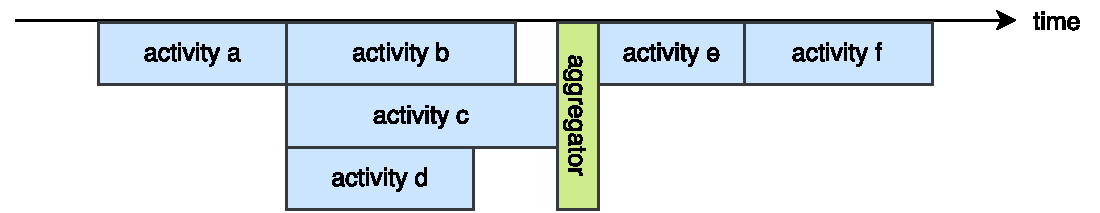
\includegraphics[width=0.9\linewidth]{gfx/figures/workflow.pdf}
\caption{A workflow with sequential, parallel, and aggregator steps}
\label{fig:workflowexample}
\end{figure}

When each step completes, an event is generated.
These events are collected from the different processors into a single database.
Each step is associated with a timestamp and all the available metadata.
The system works by a ``best effort'' delivery. 
This means the delivery of the events to the database can fail and thus be delayed.
Furthermore, the distributed system involves multiple machines in multiple locations. 
This results in variance of seconds to minutes in the clocks of the systems.
The clock variance is directly seen as noise in the timestamps of the events.

Because of the described parallelism and the uncertainties mentioned, the overall state of the system is difficult to describe at any given time.
Looking at the raw log data is also challenging because of the volume.
At the time of writing, the system produced on average 15~000 events per hour with peak times averaging in the 30~000 range.
Event filtering and visualization is necessary to find the relevant data from the noise.

\subsection{Requirements engineering}

%% description of users
% engineers, developers, working on ingestion
% first party and third party publisher release managers
% managers, PMs
In the beginning of my work the project requirements were not clear.
To understand the needs of the users, I conducted requirements engineering work.
In my research I discovered five user groups relevant to the project:

\begin{description}
\item[Developers] are the Microsoft software engineers working on the ingestion and publishing system.
\item[Managers] are the Microsoft developer leads and program managers who coordinate the developers' time and what they are working on.
\item[Publishers] are the independent creators, companies, and other third parties submitting the product packages to the store.
\item[Release managers] are Microsoft employees who have been assigned to be a contact for the largest publishing companies who develop the high-profile ``triple-A'' games and applications. 
\item[Manual reviewers] are the people working for Microsoft that do the manual steps of the product validation when necessary. This includes, for example, checking a submission for fraud or inappropriate graphics or language.
\end{description}

The needs for each user group are covered in table \ref{tab:userneeds}.
I used the ``user story'' format for documenting the needs \cite{cohn2004user}.

%% description that user needs were not fully known so they need engineering
The project was done in two cycles, with requirements engineering work done in the beginning of both cycles. See section \ref{sec:timeline} for the project timeline. 
The user needs found at the start of the second section were related mostly on the presentation and the user interface, so they did not affect the main structure of the project significantly.

%% description of initial user needs
% which?

\begin{table}[htb]
\begin{center}
\begin{tabularx}{\linewidth}{| X |}
\hline

\textbf{As a developer I want...} \newline
- to see the current status of a submission so that I can investigate issues with a single submission or product.\newline
- to see the shape of the store workflows so that I can find issues in the dependencies.\newline
- to see statistics about the activities so that I can write reports to my superiors.\newline
- to be able to customize what I see so that I can have exactly the information I care about.\newline
- to be notified of any delays in the workflow so that I can investigate issues faster.\newline
- to be notified about big issues distinctively so that I can prioritize my work.
\\
\hline

\textbf{As a manager I want...} \newline
- to have statistics of the workflows so that I can report the system performance and improvements over time to my superiors.
\\
\hline

\textbf{As a publisher I want...} \newline
- to be able to know estimated times for submission completion so that I can schedule my work day.\newline
- to be able to inquire about the status of my submissions so that I can escalate any issues that arise
\\
\hline

\textbf{As a release manager I want...} \newline
- to see the detailed status of a single product or submission so that I track it and report any issues to my superiors. \newline
- to see the big picture status for all submissions related to a single product or publisher quickly so that I can save time. \newline
- to be notified about completion of crucial steps of the workflow or any issues so that I can schedule and prioritize my work. \newline
- to be able to customize what I see so that I do not see information about products that I do not own.
\\
\hline

\textbf{As a manual reviewer I want...} \newline
- to be notified in advance when a product is heading towards a manual review so that I can schedule my work day.
\\
\hline

\end{tabularx}
\end{center}
\caption{Initial user needs found in January}
\label{tab:userneeds}
\end{table}

%% business requirements
%% need to integrate with an existing system
%% confidentiality, integrity
%% working with partners

The project also involved business requirements from Microsoft. 
The major two requirements were integration with existing systems and following confidentiality requirements.
The project was required to integrate with the existing store backend systems. 
The event collection and storing was already handled by a system called \textbf{Jury}, which is an interface to browse the products in the store and see diagnostics information from the log database.
The existing system stores the events in a database and allows the used to query the events with a SQL-like query language. 
The results were shown as a list of rows with the matching events and timestamps (see figure \ref{fig:plaineventlog}). 
The project was to integrate with this querying system to load the events from the database.
The events and the product metadata in the system contained confidential information. 
Mainly there were two terms used to classify confidential data: \textit{Medium Business Intelligence} (MBI) and \textit{Personally Identifiable Information} (PII). 
In practice, it meant that any MBI-classified information related to a product should only be shown to the publisher or the partner who owns the product.
For example, the product events should only be available to the publisher who owns the product.
However, the developers working at Microsoft should be able to see all MBI-classified information.
Any PII-classified information should be considered private and should not be visible through the interface developed in this thesis. 

%% challenges
%%  user needs not fully understood
%%  unknown parallelism
%%  unsupervised learning and adaptation
%%  both real time and statistical data are needed

There were several challenges discovered in the beginning of the project.
The system implemented in the project should be unsupervised.
This means that the system should use past data to build an understanding of the workflow without the need for a user such as an engineer to supply any knowledge beforehand.
The system should adapt to any changes in the workflow automatically.
The distributed workflows contain unknown parallelism that must be detected automatically.
Furthermore, the distributed system contains noise in the timestamps which further complicate the parallelism detection.

In addition, the system should be able to provide two different kinds of information. 
The workflow models and statistics should be built based on a long term aggregate discovered from several days worth of data,
while the system should also show the real time data for the current ongoing submissions.
These two sides of information should both be utilized in the visualization.
Lastly, requirements engineering was necessary to discover the user needs. 
This is why an iterative process was set up. 
Section \ref{sec:timeline} contains a detailed description of this process.

%% needs discovered at meetings?

%% conclusion, key goals
To recap, the key goals for the solution developed in this thesis are the ability to dynamically adapt to changes in the workflow,
the ability for the user to customize the information they need, and decoupling the solution from the specific workflow steps of the store. 
The project needs to use \emph{unsupervised learning} to build workflow models, show \emph{real-time event data} to the user based on the model, 
and use the models and the real-time data to show predictions of future events.

% %%%%%%%%%%%%%%%%%%%%%%%%%%%%%%%%%%%%%%%%%%%%%%%%%%%%%%%%%%%%%%%%%%%%%%%%%%%%%%%%
%%% Material
%%%%%%%%%%%%%%%%%%%%%%%%%%%%%%%%%%%%%%%%%%%%%%%%%%%%%%%%%%%%%%%%%%%%%%%%%%%%%%%%

\clearpage
\section{Project and materials}
\label{sec:materials}

In this section I will describe the project plan.
I will start by describing the existing systems that I was to integrate with.
Next, I will describe the data that was available to be used for the project. 
Lastly, I will describe the project schedule.

\subsection{Existing systems}

The project was to be integrated on top of existing diagnostics systems to save time and to improve the overall user experience by leveraging the system they are already familiar with.
The store has an internal monitoring tool called \textbf{Jury} for the store engineers and other users to visualize details and relationships of the products and publishers in the store.
Jury implements a user interface to query the production database for products, publishers, and events.
Jury also handles authentication, authorization, and permissions.
This is needed to preserve confidentiality of private information.

Jury includes a textual query language to filter and search the database.
The query language allows the users to query for the information that they are interested in.
The queries can be saved for later use. 
The saved queries can be used as shortcuts or ``dashboards'' for the users.
For example, a user can save a query that searches for new products published within the last 24 hours.
This query can then be used by the user to periodically check the new products.

A major goal for this project was to make use of the existing query system as much as possible.
This way the benefits like user-made views and integration with the saved queries could be re-used.
The statistics and any real-time visualizations should use the query system to retrieve the events.
When retrieving the events, the user's permissions need to be taken into account to preserve confidentiality.

\subsubsection{Azure ML}

Azure ML (publicly available at \cite{azuremlpub}) is a cloud service that offers machine learning capabilities on demand. 
They offer ready-made machine learning models in the cloud for anyone to use.
They also allow the user to provide their own code or models.
One of the major features it offers is a visual interface for machine learning called the ``Machine Learning Studio'' \cite{azureml}.
The interface allows the user to set up the data flow of their machine learning solution visually with a ''drag and drop'' model and then execute it in the cloud.

I chose Azure ML for my solution because of the accessibility, quick setup, and the multitude of ``off the shelf'' models offered.
With Azure ML I was able to take the data I had and start training models quickly without setting up anything on my local machine.

\subsection{Data}
% description of event hub
The data used by the project is a list of events. The events are the log entries generated by the distributed processes of the store ingestion/publishing system. Each store system creates events and sends them through an \textit{Azure Event Hub}. 
Azure Event Hubs are a shared event streaming platform that works as a platform-independent "front door" for all the events \cite{eventhubs}. 
The event hub is divided into several separate partitions to improve availability \cite{eventhubavail}.
Furthermore, separate partitions allow for concurrent reads of events to improve throughput.
All the processors of the store systems broadcast events into a common Event Hub.
The events are then read and processed by Jury and stored in a SQL database.
My project did not concern the event hub, instead I only read the events as they appeared in the database.

% specific description of events and how they are stored
Each event consists of a \textbf{timestamp} and some metadata. 
The event also has a \textbf{submission identifier} which identifies the trace that the event belongs to.
All events with the same submission identifiers belong to a single trace.
The event timestamp describes the exact time the event happened. 
There are also two reference fields (foreign keys) referencing the \textbf{product} and the \textbf{publisher} that the event belongs to. 
Since these references are not used in this thesis, they can be seen simply as integer type identifier fields.
In addition to these, the three other fields relevant in this research are textual (string-type) fields \textbf{Source}, \textbf{Subsource}, and \textbf{Status}.
The event type is described in table \ref{tab:event}.

\begin{table}[htb]
\begin{center}
\begin{tabular}{| c |}
\hline
\textbf{Event} \\
\hline
SubmissionId : long integer\\
ProductId : long integer\\
PublisherId : long integer\\
Timestamp : DateTime\\
Source : string\\
Subsource : string\\
Status : string\\
\hline
\end{tabular}
\end{center}
\caption{Event and its fields}
\label{tab:event}
\end{table}

The Source field identifies the event source system, such as ``Ingestion'', whereas the Subsource identifies the exact processor step withing that system. 
Thus, the Source--Subsource pair is enough to identify the exact step of the workflow which generated the event. 
The Status field contains a string describing the status of the step, such as ``Completed'', ``In progress'' or ``Failed''. 
This field can be used to reason about the duration of the events and to determine whether the event is \emph{final}. 
A final-status event means that the processor has completed the activity and will not be sending further events for the activity in question.
For example, events marked with ``Completed'' or ``Failed'' status are final.
In contrast, events with an ``In progress'' status are \emph{non-final}.
These events are fired to show that a long-running activity has been started, is still running, and hasn't failed.
An ``In progress'' will eventually be followed by a final event such as ``Completed'' or ``Failed'' with the same Source and Subsource.
The common statuses are listed in table \ref{tab:statuses}.

% methods explaining splitting and grouping of traces
An arbitrary set of events can be grouped into traces by the submission identifier field. 
Within the trace each individual step can then be identified by the Source--Subsource pair.
In a valid trace there should only be a single final event for each distinct Source--Subsource pair.

\begin{table}[htb]
\begin{center}
\begin{tabularx}{\linewidth}{| l | c | X | }
\hline
\textbf{Status} & \textbf{Final} & \textbf{Meaning} \\
\hline
Completed   & Yes & The activity was completed successfully. \\
\hline
Skipped     & Yes & The activity was not needed for this submission and was skipped. \\
\hline
Failed      & Yes & The activity was completed with an error. The activity may be retried or the whole workflow may be stopped. \\
\hline
In progress & No  & The activity has been started, is running, and will finish later. \\
\hline
\end{tabularx}
\end{center}
\caption{The common values of the status field of events}
\label{tab:statuses}
\end{table}

\subsubsection{Challenges found in the production data}
\label{sec:datachallenges}

In section \ref{sec:eventtheory} we considered the event log to be a totally ordered flat log. 
In this theoretical log each event would have a clear case identifier and its location within the flat log would correspond to the real world ordering of the events.
In theory, this case identifier and the log order can be used to split the log into traces and further order the events in each trace.
However, the production data proved to be more complex than that. 

% event hub ordering
As mentioned earlier, the event hub processors work in several partitions to improve availability.
Within a partition, the order of events is guaranteed to be stable with regards to events arriving to the event hub. 
However, there is no guarantees on the interleaving of the parallel processing of the partitions.
When the events are processed by Jury, the order between the partitions may be different compared to the event arrival order. 
Thus, the event order (the row number) in the SQL database should not be fully trusted.
Furthermore, network issues or other delays can affect event ordering. 
To combat this, each event is marked with a timestamp by the sender. 
With the timestamp the estimated ordering of events can be rebuilt when they are read from the SQL database.

% clock skew between different systems
However, the events are generated by a separate systems in parallel
Each of these systems depends on its own hardware clock, and the clock synchronization between the systems is not guaranteed to be exact. 
This means that even the timestamps may include an unknown error for up to several minutes.
Furthermore, some events may be lost because of bugs, unhandled exceptions, or outages in the system.
This means that ordering the events by timestamp includes random noise, which needs to be considered.

\begin{figure}[htb]
\centering 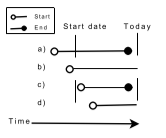
\includegraphics[width=0.5\linewidth]{gfx/figures/slice.png}
\caption{Time slice and incomplete logs \nyi{redo}}
\label{fig:timeslice}
\end{figure}

% Incomplete traces in the chosen ''slice'' (events missing from beginning/end)
Another aspect to note is that when the event log data is used, the data being analyzed is always a ``slice'' of the full event log.
This means that it contains events from a time slice starting at some time instance $t_s$ and ending at some later time $t_e$. 
All events between these times are considered. 
A common use case would be to inspect the past 24 hours of events. 
In this case $t_e$ is the current time, and $t_s$ is 24 hours earlier than the current time. 
This results in the time slice containing a large amount of events that belong to a trace that started before $t_s$.
The result also contain traces that have yet to be completed. 
This is illustrated in figure \ref{fig:timeslice}. 
These traces should be removed, since they appear to start from an event that is not a real starting point (and respectively for the end). 
Classifying a trace as anomalous like this requires an \emph{appropriate model} \cite{bezerra2009anomaly},
meaning some prior understanding is needed on how to discover whether a trace is invalid.

% resubmissions
When talking about the process mining theory (see section \ref{sec:eventtheory}) it was assumed that each trace can be uniquely identified.
This means splitting the traces form the flat event log and identifying the individual cases.
For this specific system, each submission of a product has a unique \emph{submission identifier} (submission ID).
This ID can be used to uniquely identify a trace.
However, in practice this proved more complicated.
Sometimes the application submission can be \textit{re-submitted} into the store.
This is commonly done if some part of the workflow fails to complete.
The events in such a re-submission will have the same submission ID as the original submission.
This leads to a situation where the trace seems to restart from the beginning or from a different step and continue. 
These cases should be identified as anomalous. 
In the case of real-time data, only the latest submission for each ID should be considered, since the earlier submissions are rarely relevant to the user.

Another big challenge comes from the real-time characteristics of the data. 
Because of agile practices and continuous delivery, the store systems are under constant change. 
This means that the underlying process model can change any time.
The process model generated a day before may not reflect the current state anymore. 
The system should be flexible and should adapt to any changes in the underlying models.

% invalid states
Furthermore, the production data will include also traces that have failures or phases that are in progress.
A trace with failed or erroneous steps should be considered anomalous, since a workflow is not guaranteed to progress normally after an error. 
Similarly, the traces include events that do not describe a final state, but only broadcast status. 
The most common type of event like this events with an ``In progress'' status.
If an event is non-final, it means that the same process is still expected to fire a final event afterwards.
These events should be handled differently in the modeling phase.

All these characteristics require that the system uses some kind of pre-processing method that takes the slice of the real-world data and outputs an ordered and grouped set of traces with the anomalous traces removed.

\subsection{Project timeline}
\label{sec:timeline}
% description of research timeline
% weekly meetings with manager, PM
I started preparing for the project in late 2016.
The project started in Redmond, WA, USA in early January 2017.
While the main goal of the project was established early, the details needed some research. 
For this reason, an iterative process was set up.
I held weekly meetings with my manager, as well as weekly project meetings together with my advisors and the team program manager. 
In addition, in the mid-way point I held three presentations to people from the different user groups to find more requirements and to get feedback. Because of this, the project was divided in two iterations.
The weekly meetings were carried out through both iterations.
The complete timeline of the project can be seen in figure \ref{fig:projecttimeline}.

\begin{figure}[htb]
\centering 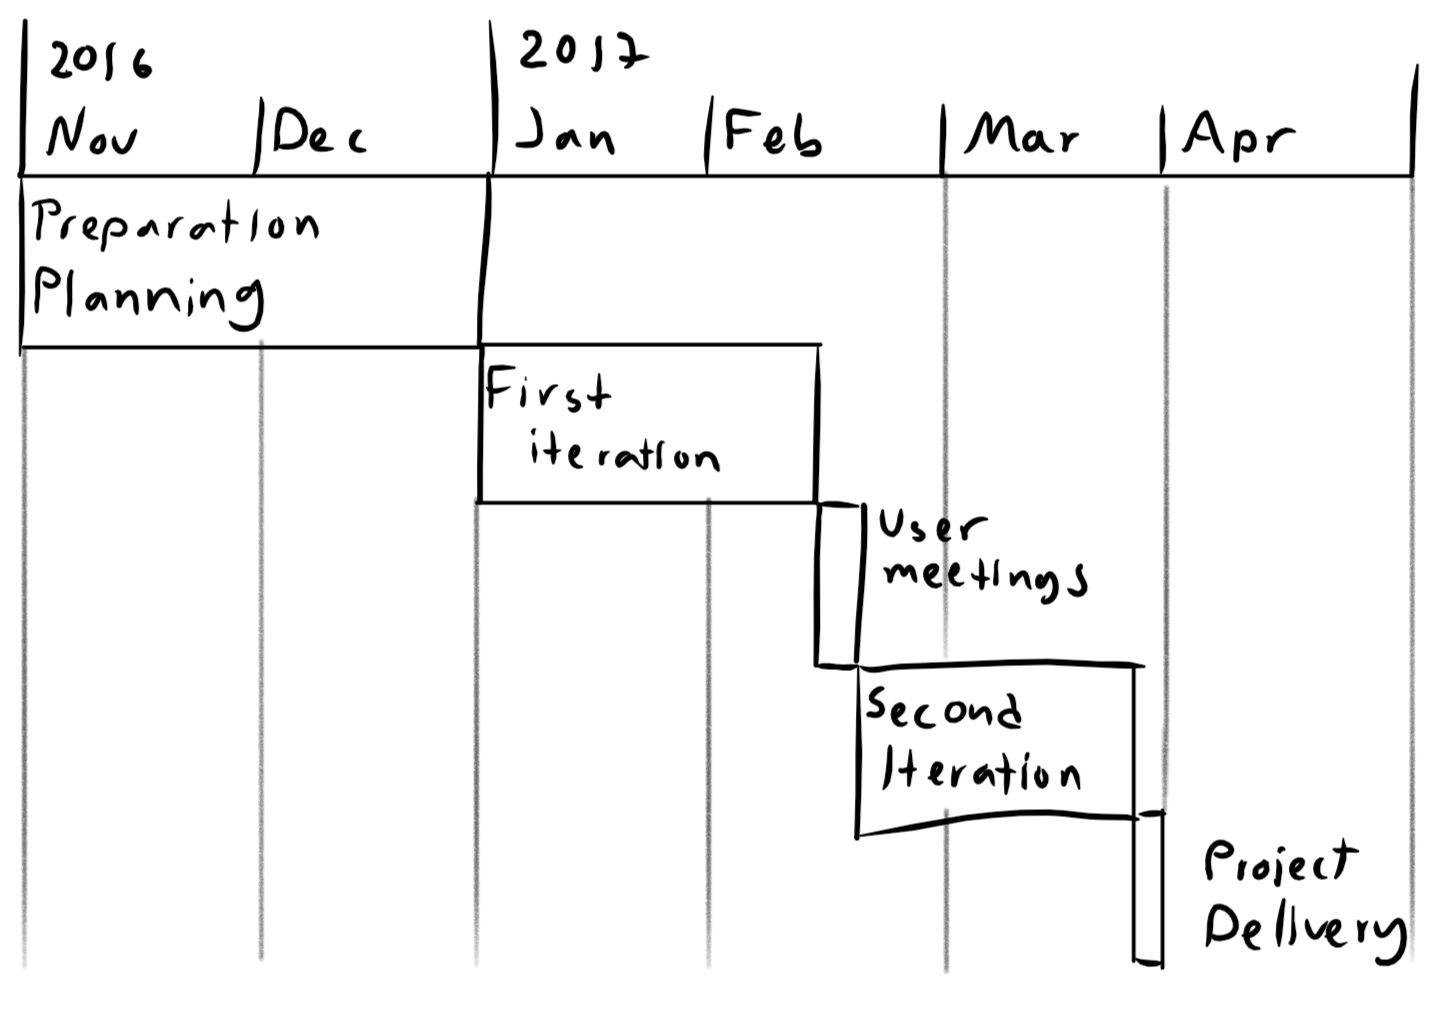
\includegraphics[width=0.9\linewidth]{gfx/figures/projecttimeline.png}
\caption{Project timeline}
\label{fig:projecttimeline}
\end{figure}

% - first iteration: supporting work, backend, graphing, initial UI
%   - explorative prototypes
%   - two UI proposals, graph and timeline
I started the first iteration by building a prototype using a small test dataset of events exported from the database. The purpose of the prototype was to explore the graph generation algorithms and to build a proof of concept. After the prototype was validate with the team I integrated it with the Jury system. I built two user interface proposals based on different types of presentation. The first one showed a directed graph describing the workflow model. The second interface showed the events on a scrollable timeline.
See section \nyi{add ref} for the detailed descriptions of these views.

% - user meetings (brownbag, 3pp)
After the first iteration I held three presentations, two of which included a feedback session with exploration for use cases. The first presentation was an open one to the higher management and the other teams. The second presentation was with the release managers to get feedback from them and to find more requirements. The third was a ``brown bag'' type of open meeting with other team members who interact with the Jury system.
In these meetings I validated my prototype designs and collected more requirements.
In the meetings the timeline view was seen more useful for most user groups.
The only exception was the engineers who saw the graph view more useful for debugging.

% - second iteration: user interface work, features to fit needs
%   - machine learning exploration
%   - graphing accuracy exploration (alt graph)
In the second iteration I spent more effort on the user interface, based on the meetings.
I experimented with machine learning models and the graphing algorithm.
Furthermore, I worked with the team to integrate the graphs with the email notification system in Jury so they could be used to send emails about delays observed in the system. 
By the end of the second iteration the project was fully integrated with Jury and was delivered to the users.
%%%%%%%%%%%%%%%%%%%%%%%%%%%%%%%%%%%%%%%%%%%%%%%%%%%%%%%%%%%%%%%%%%%%%%%%%%%%%%%%
%%% Methods
%%%%%%%%%%%%%%%%%%%%%%%%%%%%%%%%%%%%%%%%%%%%%%%%%%%%%%%%%%%%%%%%%%%%%%%%%%%%%%%%

\clearpage
\section{Methods and implementation}

To supply the required information and visualizations to the users I decided to use the process mining methods to analyze the event logs stored in the database.
I built my project into Jury, extending its functionality to provide detailed event analysis with visualizations.

I chose to use the theories from the \textalpha-algorithm to generate directed graphs describing the process model.
The graphs will be generated by analyzing several days worth of data from recent event log data. 
This way the graph dynamically adapts to change. 
Because of the several day long window the change is slow enough for the users to digest. 
However, I chose to generate the graphs based on user-supplied queries.
Hardcoded predefined values or graph shapes were to be avoided.
This way the time windows and event filters can be changed at any time without the need for a programmer to change the code.

The graphs were visualized to the users with two different views. 
The first view shows the directed graph to the user as is. 
The second view draws the graph on a timeline showing the activity start and end times.
The user can choose a previously generated model and overlay the real-time data on top of it.
Furthermore, the graph will include estimations for future events and their predicted times.

In this section I will go over the methods I used to solve the given problem in detail.
I will describe how they were implemented in the store systems.
I will also introduce the technology choices and explain how they were used to implement the methods.

\subsection{Chosen technologies}

The decision about which technologies I would use for my project was straightforward.
Since the project was to integrate with the existing Jury system, I chose to share its technologies and libraries.
Jury was built with C\#, running as an ASP.NET MVC application with .NET Framework.
The database was running on SQL Server, and the query engine was set up with an object-relational mapping tool called Entity Framework. 
\nyi{Need versions?} 
The approach used was a ``data first'' model \nyi{ref}, where the system automatically generates models (C\# classes) based on the database schema. 
\nyi{links, citations}
The user provided text queries were translated to database queries with LINQ. \nyi{elaborate?}
I used these same technologies in my project.

\subsection{Graph construction}

\subsubsection{Pre-processing}

To comply with the user requirements of being able to generate models from custom queries and real-time production data, 
the system developed in this thesis should be able to take any set of events as the input.
As outlined before, the system should use the textual query system to retrieve the events from the database.
The system will not have any knowledge of what filtering has been used, it only executes the user-given query.
The only check the system needs to do is to check the events against the current user's permissions, to protect confidential information.

The Jury system already had functionality to retrieve the events from the database based on a \emph{query}.
A query is a character sequence (a string) containing user-provided criteria for which events to show, based on the fields of the event entry (see table \ref{tab:event}).
For example, the user could be querying for a specific product or a specific submission ID.
A query ``\texttt{submissionid is 100100}'' would return all events from the specified submission.
Boolean operators familiar from search engines such as ``\texttt{and}'', ``\texttt{not}'', and ``\texttt{or}'' can be used to combine multiple conditions to form a more complex query.

After the query has been executed by Jury, the result is a set of events.
Jury displayed the set to the user as a plain timestamp-ordered list of events as seen in figure \ref{fig:plaineventlog}.
Because of the challenges outlined in section \ref{sec:datachallenges} a pre-processing step is necessary.
The plain set of events needs to be filtered and grouped into valid traces.

The pre-processing step takes a set of events as the input and works as follows:
\begin{enumerate}
    \item Drop events based on the user's permission level.
    \item Group all events by \textbf{submission ID}.
    \item Create a trace corresponding to a submission for each of these groups.
    \item Order all events in each trace by ascending timestamp, then by event ID.
    \item Drop all traces containing an event describing an error such as ones with a status ``Failed''.
    \item Drop all non-final events from each trace.
\end{enumerate}
After these steps the result is a set of \textit{valid traces} with only final events, each corresponding to a \textit{unique submission ID}.

By using different time slices or different filters on which events to include, we can generate models for different purposes. 
For example, we can try to generate a more accurate process model by filtering the events.
If we filter the events in the pre-processing step to only include events related to certain products
or product types, we can assume that the process model and the statistics will better describe those products.

However, filtering reduces the number of events used for the model, which can lead to overfitting.
For example, if the model is generated for only submissions that contain large file sizes, it may affect the results of the process discovery. 
In theory, some of the activity lengths could depend on the file size, meaning a query only containing large files may result in these activities always appear to complete later in the log.
This would result in inaccurate process models.
Because of this, care should be taken when creating models from small datasets.

\begin{figure}[htb]
    \centering 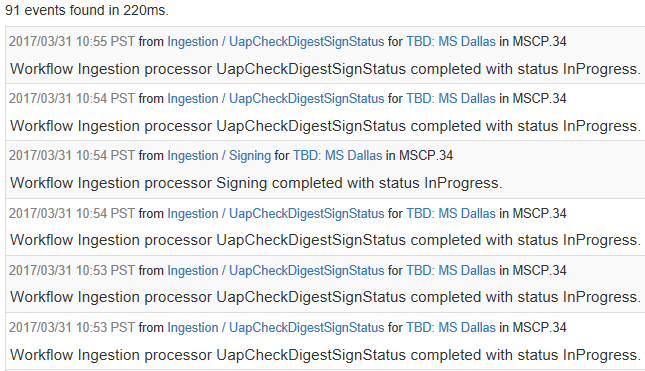
\includegraphics[width=0.7\linewidth]{gfx/screenshots/plaineventlog.png}
    \caption{Event log query result view in Jury}
    \label{fig:plaineventlog}
\end{figure}

I use the existing queries in Jury in my implementation to retrieve events from the database. 
The queries can be written by users and saved in the system.
These saved queries are then used to discover the process models.
Each model has a corresponding saved query.
For example, if the query searches for events belonging to only game products, 
then the discovered process model should reflect the underlying process specifically for games.
This allows for a highly flexible system where the users can create models for any subset of products or events that are relevant to them. 

\subsubsection{Creating directed graphs}

The model chosen to represent the process models is the directed graph. 
In this model, every pair of directly subsequent events $(a,b)$ appearing in a trace corresponds to a 
graph edge from node $a$ to node $b$.
The directed graph was chosen because of its familiarity to non-technical users since it resembles a traditional flowchart.
The parallelism is generated by observing the direct follow-relations similarly to the \textalpha-algorithm described in section \ref{sec:alphaalgorithm}.

To generate a graph from a set of traces, I started by generating an event log \emph{footprint matrix}.
The footprint matrix describes the relation of all the events in the log regarding to each other.
This means that the matrix describes which events immediately follow other events in the set of traces.
The columns and rows of the matrix correspond to all the distinct events (the event vocabulary).
The matrix is square and should have a zero diagonal, since each final event should only appear once in a trace.
The row describes the first event, and the column the event directly following.
The number in the matrix cell describes the frequency that this follow relation was observed in the logs.
This matrix is labeled the \textit{follow-frequency matrix}.
It can be generated by linearly traversing each trace once, and for each pair of subsequent events incrementing the number in the corresponding cell.

I will illustrate this with an example. Consider an event log with four activities $a,b,c,d,$ and $e$.
Figure \ref{fig:exampletraces} illustrates the six traces in the event log. There are two unique kinds of traces, $abcde$ and $acbde$, both of which have been observed three times. Figure \ref{fig:examplematrix} shows the footprint matrix generated from these traces.
The diagonal is zeroes, since no event follows itself.
Looking at the upper triangle the matrix we can see that $b$ has followed $a$ three times and $c$ has followed $b$ three times. From the lower triangle we see for example that $a$ has never followed $b$, but $b$ has followed $c$ three times.
By comparing the frequencies in the upper triangle to the lower triangle we can discover dependencies suggested by the event log, and from a lack of dependency we can suggest parallelism.

\begin{figure}
    \centering
    % example traces
    \begin{subfigure}[h]{0.4\linewidth}
        \begin{center}
        \begin{tabular}{| r | l |}
        Trace & Frequency \\
        \hline
        a b c d e & 3\\
        a c b d e & 3 \\
        \hline
        \end{tabular}
        \end{center}
        \caption{A list of example traces}
        \label{fig:exampletraces}
    \end{subfigure}
    % footprint example
    \begin{subfigure}[h]{0.4\linewidth}
        \begin{center}
        \begin{blockarray}{cccccc}
          & a & b & c & d & e\\
        \begin{block}{c(ccccc)}
        a & 0 & 3 & 3 & 0 & 0 \\
        b & 0 & 0 & 3 & 3 & 0 \\
        c & 0 & 3 & 0 & 3 & 0 \\
        d & 0 & 0 & 0 & 0 & 6 \\
        e & 0 & 0 & 0 & 0 & 0 \\
        \end{block}
        \end{blockarray}
        \end{center}
        \caption{An example footprint (follow-frequency) matrix $M$ }
        \label{fig:examplematrix}
    \end{subfigure}
    \caption{Example for traces containing events $\{a,b,c,d,e\}$}
\end{figure}

% turning the matrix into a graph
The generated footprint matrix corresponds directly to the event log based ordering relations described by van der Aalst and van Dongen \cite{van2013discovering,van2016process}.
There are four possible relations between any two events in an event log $L$:
\begin{itemize}
    \item $a \rightarrow_L b$: $b$ \emph{directly follows} $a$.
    \item $a \leftarrow_L b$: $b$ \emph{directly precedes} $a$.
    \item $a ||_L b$: $a$ and $b$ are \emph{parallel}.
    \item $a \#_L b$: $a$ and $b$ are not directly related, they are $unrelated$.
\end{itemize}

Note that $a \rightarrow_L b \Leftrightarrow b \leftarrow_L a$ is always true.
We can find these relations from the footprint matrix $M$ by comparing each cell $m_{ij}$ the upper triangle with the corresponding cell $m_{ji}$ lower triangle by using the algorithm described in definition \ref{def:logrelations}.

\begin{definition}
Let $A = \{ a_i | 0 < i \le n \}$ be a set of $n$ activities (the \emph{vocabulary}).
Let $M$ be an $n \times n$ footprint matrix corresponding to $A$.
For each cell $m_{ij} \in M$ where $i < j$:
\begin{itemize}
    \item $a \#_L b$ iff $m_{ij} = 0$ and $m_{ji} = 0$
    \item $a_i \rightarrow_L a_j$ iff $m_{ij} > m_{ji}$ and $m_{ji} = 0$
    \item $a_i \leftarrow_L a_j$ iff $m_{ij} < m_{ji}$ and $m_{ij} = 0$
    \item $a_i ||_L a_j$ iff $m_{ij} > 0$ and $m_{ji} > 0$
\end{itemize}
Furthermore, it should be noted that these relations are symmetrical:
\begin{itemize}
    \item $a \#_L b \Leftrightarrow b \#_L a$ 
    \item $a_i \rightarrow_L a_j \Leftrightarrow a_j \leftarrow_L a_i$
    \item $a_i ||_L a_j \Leftrightarrow a_j ||_L a_i$ 
\end{itemize}
\label{def:logrelations}
\end{definition}

In the example described before, comparing the cell $M[a,b] = 3$ to cell $M[b,a] = 0$ results in $a \rightarrow b$.
However, by comparing $M[b,c] = 3$ to $M[c,b] = 3$ the algorithm results in $b || c$. 
Figure \ref{tab:examplefootprint} shows the generated footprint for the matrix shown in figure \ref{fig:examplematrix}.
Note that it is enough to only examine the upper triangle of the matrix, since the generated footprint is always symmetrical across the diagonal.
If the rows and columns are ordered by dependency, the dependencies follow the diagonal of the footprint.
The parallel activities can be seen visually as square-shaped symmetric regions.
The parallel region border consists of follow-relations while the inside of the region contains parallel-relations.
This shape can be seen in the example figure \ref{tab:examplefootprint}.

This footprint maps directly to a corresponding directed graph.
Every activity in the vocabulary corresponds to a graph node.
Every ``directly follows'' relation corresponds to a directed arc (edge) in the graph. A parallel relation corresponds to arcs in both directions.
Figure \ref{fig:examplegraph} shows the directed graph corresponding to the footprint from figure \ref{tab:examplefootprint}.

\begin{figure}
    \centering
    % footprint table example
    \begin{subfigure}[h]{0.4\linewidth}
        \begin{center}
        \begin{tabular}{cccccc}
        \hline
          & a & b & c & d & e\\
        \hline
        a & \# & $\rightarrow$ & $\rightarrow$ & \# & \# \\
        b & $\leftarrow$ & \# & || & $\rightarrow$ & \# \\
        c & $\leftarrow$ & || & \# & $\rightarrow$ & \# \\
        d & \# & $\leftarrow$ & $\leftarrow$ & \# & $\rightarrow$ \\
        e & \# & \# & \# & $\leftarrow$ & \# \\
        \hline
        \end{tabular}
        \end{center}
        \caption{Generated footprint of log relations}
        \label{tab:examplefootprint}
    \end{subfigure}
    % directed graph example
    \begin{subfigure}[h]{0.4\linewidth}
        \centering 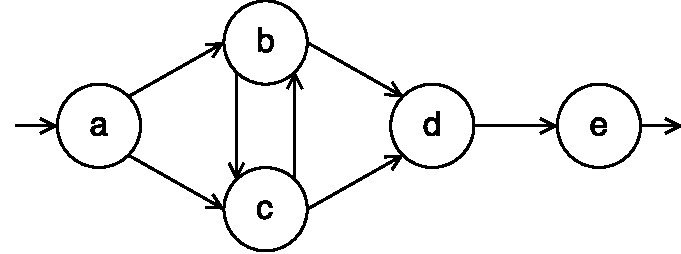
\includegraphics[width=\linewidth]{gfx/figures/graphthing.pdf}
        \caption{Generated graph}
        \label{fig:examplegraph}
    \end{subfigure}
    \caption{Graph generation from the footprint}
\end{figure}

% Dealing with noise
Noise in the event log data creates problems if it is not appropriately handled. 
Network delays, bugs, and other errors cause events to get lost or erroneously arranged in the traces. 
This noise manifests in the footprint follow-frequency matrix.

Figure \ref{fig:examplenoise} shows an example footprint matrix from a slice of production logs.
The frequencies shown in the figure are logarithmic for improved visibility.
As can be seen from the figure, two parallel regions of activities can be seen clearly in the data.
The first region contains three parallel activities, and the second one seven activities.
Within the regions, the frequencies observed are fairly constant.
However, outside the regions most cells still have non-zero values, even though the real process model
does not have parallelism between the leftmost and the rightmost activities.
This is the aforementioned log noise.
If left as is, the noise will create invalid arcs in the graph.

\begin{figure}[htb]
    \centering 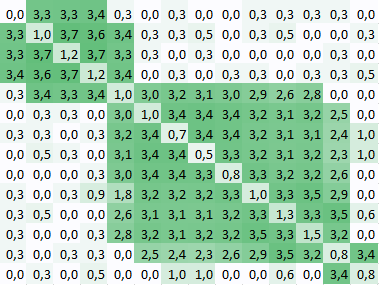
\includegraphics[width=0.6\linewidth]{gfx/graphs/noise.png}
    \caption{Observed noise in production data (logarithmic scale)}
    \label{fig:examplenoise}
\end{figure}

My method of dealing with the noise was to apply a threshold value to all the frequencies.
The value was a fraction $0 \le t_n < 1$ of the number of traces $N$ analyzed in the event log.
Any value in the matrix lower than $t_n N$ will be set to zero before the matrix is turned into a graph.
Similar thresholding will be performed when checking for parallelism (see definition \ref{def:logrelations}). 
For parallelism I calculate a fraction $d_p = \frac{f_\text{follow}}{f_\text{follow} + f_\text{precede}}$, where $f_\text{follow}$ is the frequency of follow relations from the upper triangle of the footprint matrix and $f_\text{precede}$ is the respective frequency from the lower triangle.
To counter noise, the relation is only considered to be parallel if the fraction is between the treshold values $t_p \le d_p \le (1 - t_p)$. 

Initial tests on the production data showed that relatively small ($t_n \le 0.01$) values were sufficient to counter the noise without affecting the model negatively. 
I used $t_n = 0.01$ and $t_p = 0.005$ to remove 1~\% of noise.

\nyi{Add figure for observed relations from excel}

% directed graph tldr
The result of this method is a directed graph with nodes and edges.
The graph describes the process model that was discovered from the event log.
Each node corresponds to an activity in the process model.
Each edge corresponds to a possible transition (pair of two consecutive events) in the trace.
The model can be verified by ``re-playing'' a trace as described in section \ref{sec:processmodelsdsc}.
Each event in the trace should correspond to a valid directed edge, with the first event of the trace being at the input node of the graph.

\subsubsection{Latency}
\label{sec:latency}

In addition to discovering the process model, one of the requirements was to see statistics of the times each of the activities take. 
Since the event timestamps describe the end time for each activity, the length (or duration) of an activity can be found by comparing the timestamps of two consequent events. 
I call this time difference between events the \emph{latency}.
The latency describes how much time is expected to pass until an event is followed by another event.
The latency can be seen as the length of an edge in the directed graph.

The statistics the users were interested in were the ``top percentiles'' (TP).
A top percentile is a value that corresponds to a set of numbers, such as all the observed durations of activities.
A $n$-top percentile means the value that is higher or equal than $n\%$ of all the values in such a set.
This can be expressed as the ``TPn'' value.
For example, the TP75 is the value that is higher or equal than 75~\% of all the values in the set.
TP50 corresponds to 50~\% and is equal to the median value of the set.
When looking at statistics about the store, the top percentiles have proven to be useful.
Looking at average values is often misleading, since the store systems often contain a very small amount of outliers with very high latencies, that skew the averages up.
The interesting statistics that were chosen are the TP50, TP75, and TP90. 
These correspond to the values used in other telemetry systems so they can be compared against for verification purposes.

In practice the TP values can be found by ordering the values in the set in an ascending order as an array, and then picking the index that corresponds to the percentile. For example, is the ordered array has the length of 1000 elements, the TP90 value can be found at the 900th index of the array.

My method was to collect the statistics at the same time as generating the graphs.
Since each cell in the footprint corresponds to an edge in the graph, I construct an array of latencies for each cell as I traverse through the traces.
When a number in the follow-frequency matrix is incremented, I also store the latency between the two events in the corresponding array. 
After the graph is generated, I can store the chosen key statistics (TP50, TP75, TP90) for each graph edge and discard the matrix and the arrays.

\subsubsection{Loading graphs from a file}
\label{sec:jsonfile}

As a secondary option, I developed a method to bypass the graph generation algorithm completely, and instead load the shape of the model from a JSON (JavaScript Object Notation) definition file.
By using a definition file, the engineers can ``force'' a template to have a specific exact shape.
This is useful in a few applications.
In some cases it is useful to have a ``stable'' graph with a pre-defined shape.
Since the algorithm is unsupervised and train itself constantly with a multiple day time window (e.g. the last 7 days), any changes made into the process may take the same time to become visible in the graph.
Additionally, small datasets can be too noisy for the algorithm to correctly identify the shape.
In such cases, the engineer can supply a JSON file.
This only affects the graph shape discovery. 
All the other parts of the systems work identically for both cases.
This feature can be toggled on a template by template basis, so both JSON-defined and automatically generated templates can be used side by side.

\subsubsection{Paging}
\label{sec:paging}

% implementation, paging
Many queries can return hundreds of thousands of events and visualizing all of them would be resource-intensive.
In addition, when discussing the requirements with the users they often only wanted to see the latest few submissions.
Because of these reasons I developed a paged view that visualizes the events retrieved from the user's query, but restricts the number of graphs shown to the user in a predictable way.

First, I run the user's query and retrieve the events, filtered by the user's permission level.
I sort these events by descending timestamp and pick the five latest submission IDs.
These IDs will correspond to the five latest submission traces matching the user's query.
``Latest'' in this context means the traces with the most recent activity.
Optionally, the user may select to see the traces ordered by the latest start time.
This query may also be paged, allowing the user to choose the next five traces, or any later set of five.
After five submission IDs has been retrieved, they are used to query all events belonging to these submissions. This results in five traces that can now be processed.

This is implemented with two SQL queries.
The first query that retrieves the five submissions can be paged with a standard page selector user interface component.
This means that the user can choose to see the next ``page'' of submissions containing submissions 6-10 and onwards.
The first query uses a \texttt{GROUP BY} clause to group the events by submission ID and to choose the maximum timestamp.
This result is then sorted and the top five IDs are selected.
This selection can be paged with a SQL \texttt{OFFSET} clause based on the user's page selection.
The query runs in only a couple seconds on a cloud-hosted SQL Server instance.
The second query retrieves all events that belong to the retrieved five submissions.
These events are then passed to the graph generation algorithm.

\subsubsection{Storing the graphs}
\label{storinggraphs}

As described before, the project allows the users to generate new graphs from any query supplied by the user.
Reading hundreds of thousands of events from the database, sorting them and generating the graph takes a lot of time, in the order of several minutes.
Creating new graphs from a previously unseen query is resource-intensive, so the functionality is restricted to the system administrators in Jury. 
Since Jury is an online tool the service response times need to be fast, preferably in the order of a fraction of a second, to preserve a smooth user experience \nyi{cite?}.
Generating the graph from a set of events for each web request from any user would be inefficient and the page load times would be in the order of minutes.
Because of this, I implemented two levels of caching in the system.

The Jury web server is distributed onto multiple server instances to provide high availability. The database server is shared between the instances.
Each generated graph is cached both in the database and locally in memory at a server instance.
The in-memory cache is local to each instance and the database cache is shared.

Each cached graph is associated with a timestamp corresponding to the time when it was generated. 
This timestamp is used by the servers to determine when the cache is too old and should be refreshed.
For the in-memory cache this maximum age was chosen to be 15 minutes.
For the database cache the maximum age was set to 12 hours.
The long time was chosen to be sufficient for the store backend system.
While the process model of the store system changes constantly when improvements are made, the changes happen over several days rather than hours. A day old cached model will be accurate in most cases.

The cache system works as follows (from the perspective of a single server instance):
\begin{enumerate}
    \item The server receives a HTTP request requiring a specific graph.
    \item The server reads the timestamp (age) of the in-memory cache. \\
    \textbf{Graph not in memory}: Continue to the next step.
    \textbf{Less than 15 minutes old}: Return the graph from memory to the user and stop. \\
    \textbf{Older than 15 minutes}: Return the graph from memory to the user and continue to the next step in the background.\\
    \item The server reads the timestamp (age) from the graph stored in the database.\\
    \textbf{Less than 12 hours old}: Load graph from the database, store it in memory. Return to user if needed.\\
    \textbf{Older than 12 hours or not in database}: Move the graph timestamp in the database 15 minutes forward and generate a new graph. Once the task is finished, save it in the database, and in memory.
\end{enumerate}

If the requested graph is in memory, it will be returned to the user immediately. 
If the version in memory is too old, a background task to retrieve or generate a new graph is started. 
The graph in memory is returned to the user regardless. 
This means that the user almost never has to wait for the page to load while the graph is being generated.
The only case when the user has to wait for the graph generation is if the instance has no graph in memory and the version in the database is also too old.
In practice this will only happen after a server restart when all the in-memory caches are purged.

The graph timestamp is moved 15 minutes forward at the start of graph generation to prevent a situation where two different server instances are generating the same graph separately.

This two-level caching improved the page loads from minutes to fractions of a second. Furthermore, since the graphs are now stored also in the same database as the events, they can be used in SQL queries. This proved to be useful, since SQL queries can be constructed to improve the notification functionality. See section \ref{sec:notifications} for more details about notifications.

\subsection{Real-time functionality}

Until this point I have considered the case of the event log that corresponds to a time slice of past data.
This type of data can be seen as an ``aggregate'', since it will result in a model that describes events over a long period of time.
However, a key part of the analytics for the store is the ability to analyze and debug the current state of the system.
Without such functionality it will be difficult to analyze the state of the current submissions in the system.

As outlined before, the system already had a view to list events based on the user's query, as seen in figure \ref{fig:plaineventlog}.
I call this the \textbf{log view}.
The users of the system reported that this view was useful for debugging a specific issue for e.g. with a specific activity, but it does not provide a good overall view.
The request from the users was a view that would show a big picture of the status of a submission with the option to drill down to the details.

% new small dataset from a query, often a single trace
My solution was to leverage the previously discovered aggregate model for visualization.
The model would be combined with the list of events returned by the query.
The aggregate model would be used to visualize the process, and the real-time data from the query would be ``overlayed'' on top of the model.
In other words, the idea was to ``color'' the model with the real-time data from the query.

The query returns a set of events that corresponds to the user's criteria.
For simplicity we can assume that the result is a single trace for an ongoing submission,
a set of sequential events that all belong to a single case.
In the final implementation the result can also be events from many separate submissions.
The system handles it by splitting them into separate visualizations and then handling each one of them as a separate case.

In the beginning we create an ``colorless'' graph by copying the process model discovered earlier.
The colorless graph has a node for each activity and the corresponding graph edges between them.
The nodes are tied to the specific activities by including the Source and Subsource fields. 
These colorless nodes have no status, timestamp, or other metadata.
The visualization is ``colored'' by traversing through the trace in sorted order (ascending timestamp).
For each event in the trace, I find the corresponding node in the graph.
It is then ``colored'' by copying the status, timestamp, and other metadata from the event to the node.
This can be repeated until we reach the end of the trace.
The result is a ``colored'' graph where all the activities that have been finished have a status and a time.
The nodes for the activities yet to come remain uncolored.

\nyi{Does this need an illustration?}

This graph can now be shown to the user.
The nodes are drawn on the screen as circles or rectangles, and the directed edges as arrows between them.
This is what I call the \textbf{graph view}.
The parallel nodes are connected by double-sided arrows or an edge that otherwise indicates the parallelism.
In my visualization I took the ``colorization'' quite literally by having each status correspond to a real color shown to the user.
Uncolored nodes remained grey, completed nodes green or blue, nodes in progress yellow, and failed nodes red.
The colors help the user to get an immediate understanding of what the state of a submission is.
An example of a colored graph can be seen in figure \ref{fig:coloredgraph}.

\begin{figure}[htb]
    \centering 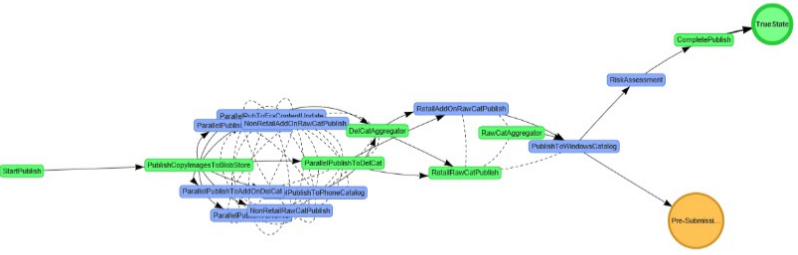
\includegraphics[width=0.9\linewidth]{gfx/screenshots/graphcolor.png}
    \caption{Colored graph view}
    \label{fig:coloredgraph}
\end{figure}

In my implementation I had to add one hard-coded aspect to cover an edge case. 
In the store system, it is possible for a publisher or a developer to ``re-publish'' a product. 
When a re-publish is triggered, the publishing steps of the workflow are run again with the same submission ID. 
This means that a trace from a single submission may contain several publishes.
My implementation detects when the first step of the publishing workflow is seen a second time in a single trace. 
When this happens, the trace is split into two and the re-publish will be shown as a separate trace in a separate visualization.

\subsection{Estimating the future}

One of the requirements discovered (see table \ref{tab:userneeds}) was to be able to provide estimations for the submission workflow completion times (labelled \emph{estimated time of arrival} or ETA). 
To provide such estimates I developed a method to traverse the graph forward after it has been colored.

% Estimating future on incomplete logs
The algorithm used in the project was a recursive traversal by using a stack.
The input for the algorithm is a graph which has been partly colored by a trace.
This means that some of the graph nodes have timestamps and metadata, while others (towards the end of the workflow) do not.
The goal is to use the previously generated process model to estimate
and fill in the data for the uncolored nodes.

% Statistical approach by using TP75
To fill in the data for future nodes, the algorithm needs a measure to be used for the estimation. 
This measure corresponds to the estimated ``edge length'' for each edge in the graph.
A simple approach is to use the statistical values that were collected during the graph generation process (see section \ref{sec:latency}).
The statistics are useful since the users prefer a ``worst case'' estimation rather than a ``best case'' one.
If a workflow finishes earlier than estimated, it is seen as a positive surprise by users.
For example, using the TP90 value should lead to an estimation that estimates the latencies in a way that overestimates 90~\% of the submissions.
However, choosing the right statistic is challenging.
The choice is a trade-off between avoiding underestimation and making an accurate prediction.
The plan was to use machine learning to improve the estimations (see section \ref{sec:ml-estimation}).

\nyi{pseudocode?}

\subsubsection{Estimation algorithm}
% algorithm description
First the algorithm finds the node which has the earliest timestamp.
This is treated as the graph start.
An empty stack is initialized and the start node is pushed into the stack.
After this initialization a recursive step is executed in a loop until the stack is empty.
In theory, since all the graphs are workflow graphs no loops should appear in the graphs (see ``connectedness'' in section \ref{sec:processmodelsdsc}). 
In practice, aspects like noise, errors, and changes in the system can lead to invalid graphs containing loops.
An empty list is initialized to keep track which nodes of the graph have already been visited.
The purpose of the list is to prevent a loop in the graph causing infinite execution or a stack overflow.

The recursive step starts by popping a node (called the \emph{current node}) from the stack and checking if the node is valid.
Validity means checking that the node has not been visited already, that the node is not an error state, and that the node has a timestamp.
If the node has been visited already it is ignored.
Error states are seen as anomalous and since they often lead to the workflow being aborted they should not be used for estimations.
The node needs to have a timestamp, otherwise there is no reference point for calculating an estimation.
After the node has been deemed valid, it is marked as visited.

After the initial check all children for the node are retrieved.
This means finding all the edges that have the current node as the source, and collecting the nodes that the edges point towards.
For each of these nodes, the estimation is performed.
If the child node already has a timestamp from the coloration phase, it is ignored.
Otherwise, if the node is uncolored, the previously chosen edge length measure (such as the TP75) is used for the estimation. 
The length of an edge is a length of time (a time span), corresponding to an estimate for how much time will pass between the two events.
By adding the time span to the timestamp of the current node, we get the estimation for the timestamp of the child node.

For parallel nodes (the nodes with a directed edge both to and from the current node) the step differs slightly. 
Since the activity corresponding to the node is known to be parallel to the current one, the edge length is seen as zero.
For this reason, the estimation step does not add anything to the timestamp but instead just copies the current node's timestamp to the parallel node.

After the timestamps of the child nodes have been estimated the child nodes are added to the stack and the step is performed again.
This continues until the stack is empty.
The stack will be empty when all the nodes connected to the starting node have been visited.
This means that, barring error states, every node will now either be colored or have a timestamp estimation.
These estimations can be shown to the user when the graph is visualized.

\subsubsection{Timeline view}

During the protyping phase I discovered that the directed graphs were not intuitive to read for the users.
Trying to manipulate the graph shape and selecting each node to see the details turned out to be cumbersome to the users.
Two users wished for a ``sorted'' view in the initial tests.
The sorted view should show the events arranged by time horizontally across the screen.
This resulted in the second prototype which I labelled the \textbf{timeline view}.
A basic example of what a timeline is can be seen in figure \ref{fig:basictimeline}.
The timeline has items set on a horizontal axis.
The horizontal axis corresponds to time, with past being on the left and the future on the right.
The vertical axis has no meaning other than to separate the parallel items visually to help the user see which activities happen in parallel.

\begin{figure}[htb]
    \centering 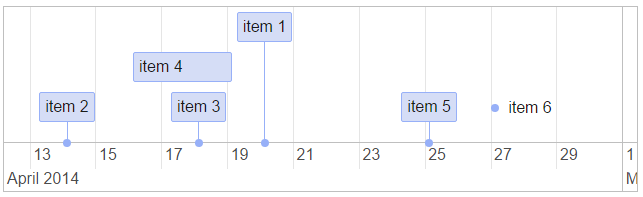
\includegraphics[width=0.6\linewidth]{gfx/screenshots/basictimeline.png}
    \caption{A basic example of a ``timeline'' \nyi{make a better one}}
    \label{fig:basictimeline}
\end{figure}

% Generating a timeline view with start and end times from the overlay
As can be seen from figure \ref{fig:basictimeline}, each item in the timeline has a width.
This means that the items have a both a \textit{starting time} and an \textit{ending time}.
However, in the event log each event only has a single timestamp corresponding to the ending time of an activity.
Since the event logs do not have any information about the starting times, the only option is to make an estimation.
To find the estimated starting times, I leveraged the process model graph again.

% Methods of finding the start times and dealing with parallelism
In my project I made the assumption that switching tasks takes a negligible (zero-length) time.
This means that when a task ends, the next task begins immediately.
With this assumption I can discover the starting time by looking at the end time of a previous task.
I can find the previous task by following the graph edges backwards and finding its dependencies.
The estimated starting time of the activity is the latest ending time of these dependencies.
In this method, all parallel tasks are treated equal, so each activity also must take into account all dependencies of its parallel tasks.
In the case where there are no dependencies (such as the first activity of the graph) a predetermined length will be used as a fallback.

In other words, before estimating the start times the timeline has all events as zero-width having only the activity end times. The algorithm sets the start time to be the earliest possible time without breaking the restrictions given by the process model dependencies.
After this step, all items in the timeline correspond to an activity and have a start time and an end time.
When the timeline is visualized the items can be separated by color (or other means) to distinguish between real-time information and estimations.
Furthermore, since the horizontal axis corresponds to time, the current time of the user can be shown as a vertical line.
This helps to highlight the current time to the user and to separate future estimations from observed events.

\nyi{add picture of a finished timeline}

\subsection{Machine learning}
\label{sec:ml-estimation}

% How ML approach could be used to improve the statistical approach
After I had implemented the statistical estimation, the next step was to research whether it could be improved by using machine learning. 
The idea was that for each graph edge, instead of using a statistical value to estimate the length, a machine learning model could be used.
The model could take into account the current time and transition, in addition to other characteristics of the submission such as details about the application package.
The hypothesis was that characteristics such as the package size have a predictable effect on the latencies.
To test this hypothesis I collected a set of training data from the production environment and used it to train and test machine learning models.
Had the model accuracy been proven to be more accurate than the statistics, the model could have been deployed to the production system.

% Explain models used (poisson \cite{azurepoisson}, bdt \cite{azurebdt} \cite{lambdamart2010})
% data suitability
% result interpretation
The machine learning models used in training were Poisson Regression \cite{azurepoisson} and Boosted Decision Trees \cite{azurebdt}.
These two were used as alternatives and they were compared against each other.
The better performing model was to be used in the final product.
These two models were chosen for testing based on a few factors.
The first factor was that the model needs to suit the data.
Since the latencies are based on the probability of an event happening, they fall on a Poisson distribution. 
This is why a Poisson Regression model was selected.
The Boosted Decision Trees model had been used before in the store for application classification with good results, so it was believed to work well with the feature set that I had available for the applications.

Second factor for choosing the models was the ability to interpret the results.
Since this project was experimental and there was no baseline, I wanted to be able to inspect the models and reason about their characteristics.
Since both the Poisson Regression model and the Boosted Decision Trees output the per-feature weights for the model, they can be inspected and reasoned about.
Compared to something like a neural network, which is highly challenging for humans to interpret \nyi{citation needed} this is a clear advantage.
The best model based on prediction accuracy was to be chosen for an in-production test.

% accuracy
% training / regression speed
Mean absolute error and the mean square error values were to be used to evaluate model accuracy.
Lastly, if multiple accurate models was to be found, the model training and regression performance would be used to evaluate them.

\subsection{Feature set}
\label{sec:featureset}

% Explain training dataset generation
The training dataset was generated from a time slice of the event logs. 
By using both a predetermined process model by using a JSON file (see section \ref{sec:jsonfile}) and the automatically discovered process model, two datasets were created. 
The datasets will be referred to as the ``JSON template'' dataset and the ``Automatically generated template'' from now on.
The datasets contain the observed values for the latencies, labelled by the activity transition and the application it belongs to.
These rows were then joined with a dataset of known applications and their characteristics to create the final training data.
The resulting dataset consisted of 16 columns of features such as the package size and the current transition (activity being observed), and a label column corresponding to the measured latency in seconds. 
See table \nyi{ref} for an example.
The data was filtered to only contain measurements from valid traces with the requirement of having no errors and conforming to the process model.
The datasets and their headers were anonymized before they were used to train the models.
Any information identifying a specific product was removed.
Furthermore, the column headers were replaces with generic ones, since the name of a column does not affect the result of the training.
The datasets used contain 36~982 rows for the JSON generated template, and 18~860 rows for the automatically discovered template.
The data reflect three days of event log data.

\nyi{Add table with example rows}

% Explain initial testing
% Testing with noisy features removed (textual fields)
The features used in the data were chosen based on experimental testing and domain knowledge.
Initially, data included fields such as the application description, keywords, and other developer-supplied textual information. 
However, these were deemed noisy and they drastically increased the training time because they required n-gram generation.
The domain experts (the system engineers) knew to inform that those fields are not used in the ingestion pipeline so they were removed from the datasets.
After the removal 12 features read from the application package characteristics where used. 
The data included numeric features such as the package size in bytes and some count data from the store related to how many previous submissions the application has.
There were also binary (true or false) features describing characteristics of the package, such as what kind of hardware permissions the application needs to have.
The two features read from the event logs were the current time in seconds since the submission start, and an enumerator for the current transition (the activity in question).
The label column was the latency (the duration of the activity) measured from the event log.

% Explain additional features
% identical resubmission
After the initial testing, two additional features were added to the dataset.
The first additional feature was a boolean value describing whether the application package is identical to the previous submission.
This was because the domain experts knew that this would lead to some of the activities skipping execution internally, drastically reducing the execution time for a couple specific activities. 
This was also clearly seen in the data when the latency distribution for an activity were plotted. 
Figure \ref{fig:resubmissions} shows that there is a clear divide between two sets of latencies.
The lower set of latencies are caused by the system detecting an identical submission and skipping the activity.
With this graph the training data could be split into two sets labelled by whether the submission is an identical resubmission.
%  posting that needed human interventiondcxfkkkkkkkkkkkkkkkkkkm
%                                       a cat did this ^ 
The second additional feature was whether the application ingestion triggered a manual review (human curation). 
Since orchestrating human manual reviewers contains overhead, a manual review is known to delay the ingestion time considerably.
This can seen from a latency distribution graph as a clear difference for the steps related to curation. 
Figure \ref{fig:manualreview} shows this effect in the distribution of the curation latency.
This knowledge was used to add the manual review boolean feature into the dataset.
I performed more tests with these two additional features to test whether they improved model accuracy.

The best performing models within a model class (such as the BDT) were found by running multiple models with different parameters in parallel and choosing the model with the best performance.
Initially the models had random (or default) parameters.
After the parallel tests the best performing model was selected as the baseline for the next iteration and the next set of models.
The iteration was repeated until better performed models could not be found anymore.
The resulting parameters and their error values from the tests can be found in section \ref{sec:results}.

\begin{figure}[htbp]
    \centering 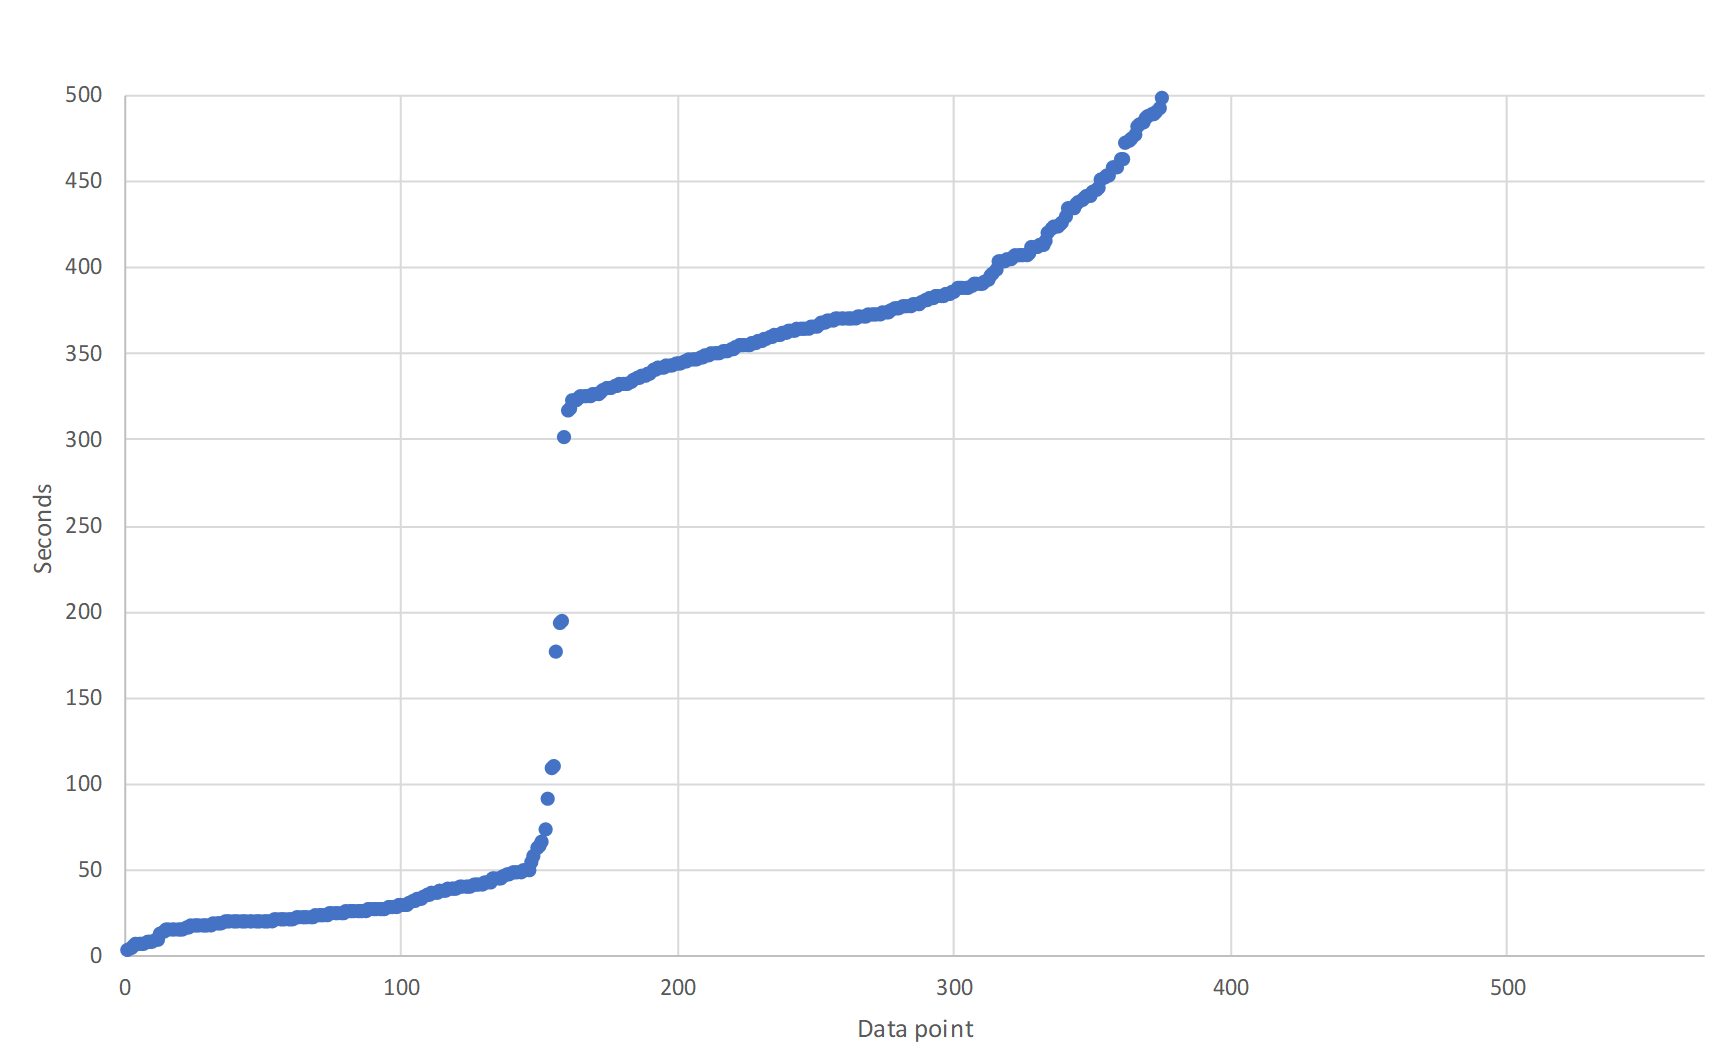
\includegraphics[width=0.9\linewidth]{gfx/graphs/resubmissions.png}
    \caption{Latency distribution divide caused by re-submissions}
    \label{fig:resubmissions}
\end{figure}

\begin{figure}[htbp]
    \centering 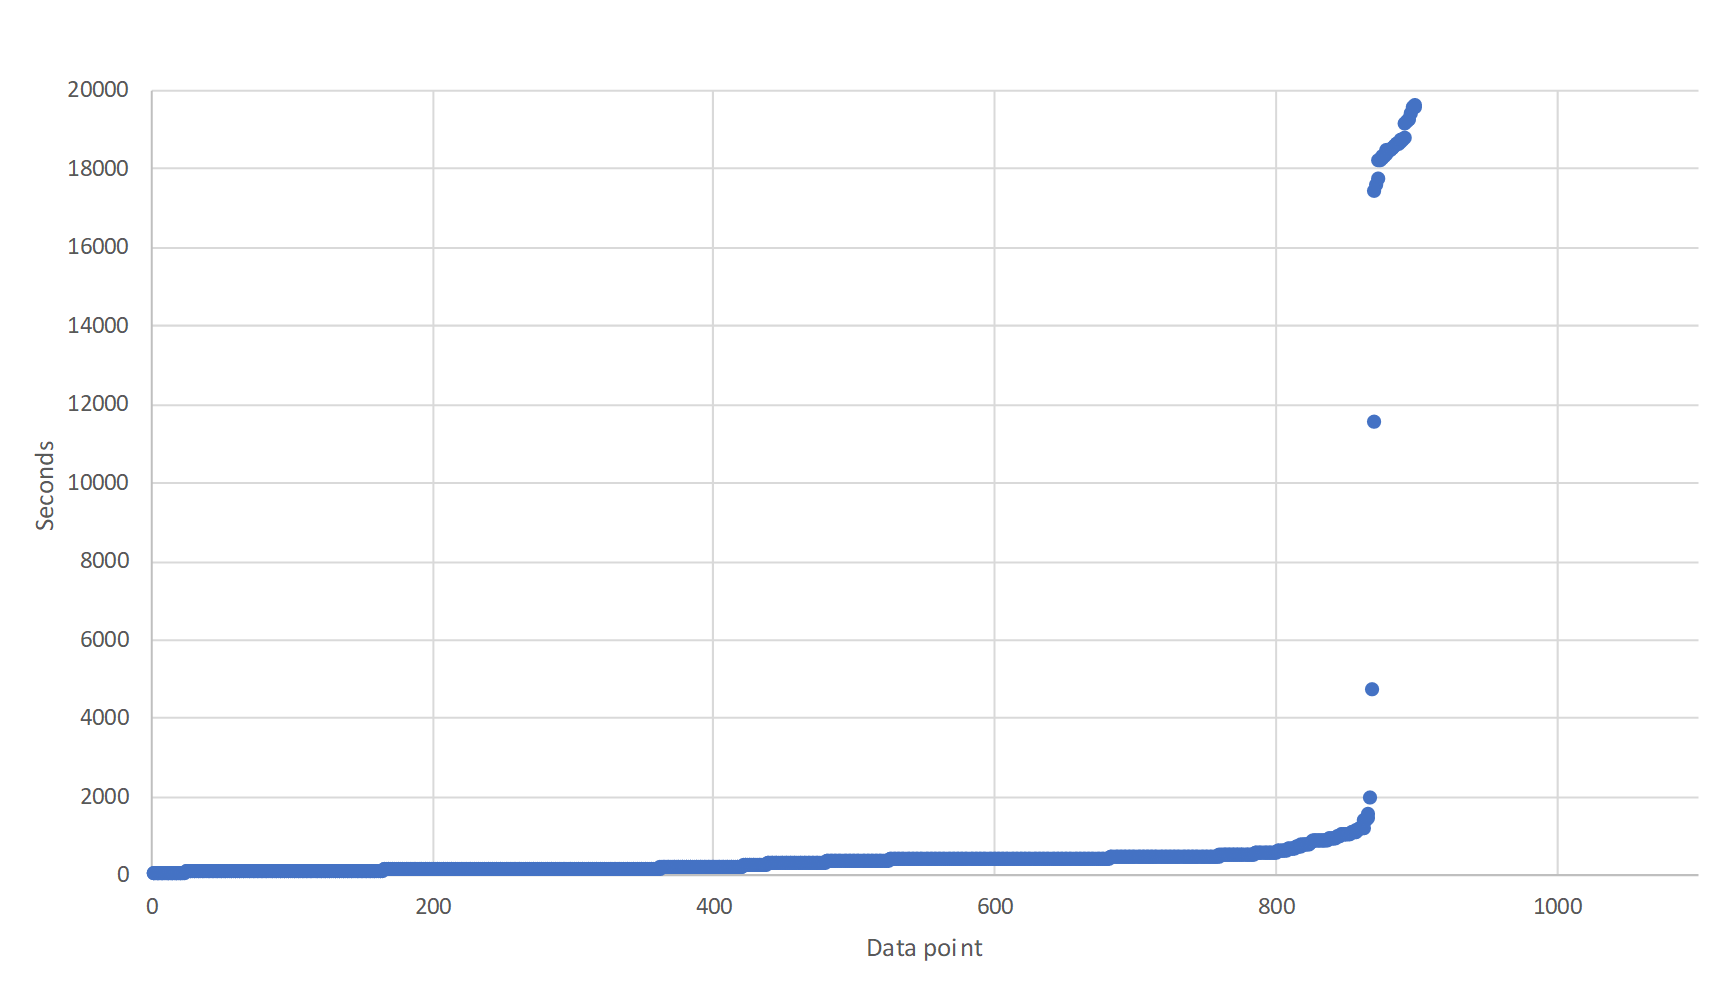
\includegraphics[width=0.9\linewidth]{gfx/graphs/manualreview.png}
    \caption{Latency distribution divide caused by entering manual review}
    \label{fig:manualreview}
\end{figure}

\subsection{Notifications}
\label{sec:notifications}

One of the main features of Jury is the ability for the user to request notifications for any events that are relevant to them.
The users can run queries and ``subscribe'' to them.
Whenever an event arrives to Jury which matches a subscribed query, a notification such as an email is sent to the user.
This allows Jury to notify the user for example when a product they are interested in receives an update or when an error happens.
Because the notifications use the same queries as the other parts of Jury, they allow the same high level of customization.

However, notifications were only triggered as a response to an incoming event.
This means that if an event was missing or delayed no notification could be sent.
Similarly, no notification could be sent about a workflow activity when it started, only when it was completed.

Receiving notifications for delayed submissions was a requirement discovered from users (see table \ref{tab:userneeds}).
Furthermore, notifying about a workflow activity before it happens was seen to be useful for scheduling purposes.
This functionality, or the data required for these functions, was not available in the old Jury system.
However, after I cached the process models and their statistics in the database (as described in section \ref{storinggraphs}) this data was now available in the same database as the events.
This allowed for SQL queries to be created to detect when an event is ``late'' before it even arrives.

For detecting late events, the system needs to examine the current ongoing submissions and the events that have been received already.
The submissions and their latest events can be found with a \texttt{GROUP BY} query as described in section \ref{sec:paging}.
In addition, each transition (graph edge) in a process model is associated with its statistics. 
This means that when the edge is stored in the database it also contains numeric values for the statistics such as the TP50, TP75, and TP90 (see section \ref{sec:latency}).
The latest event and the process model can be used to find the next expected transition for each event.
I did this by joining the latest events with the process model graph edge that corresponds to that event.
By adding the time span from a chosen statistic (such as the TP75) to the timestamp of the event I form an ``estimated time of arrival'' (ETA) for the next expected event.
If the current system time is past this ETA, we know that the next event is currently ``late'' and should have already been received based on the statistic chosen.

% tolerance, absolute and statx2
Because of the natural randomness and varying small delays in the system, choosing a good statistic is crucial. 
For example, if I used the TP75 as the statistic for late event notifications, even in the ideal case the user would be notified 25~\% of the time.
Furthermore, the users generally are not interested in event being very slightly late (such as a couple minutes) but only after the event is ``considerably'' late.
What ``considerably late'' means should be chosen by the user, not the developer, since the user is the domain expert.
Similarly, some activities are very short in length so even a one minute delay caused by the clock skew can seem like a large relative delay.
In addition, some activites may involve absolute contractual SLA times that are critical and should not be based on statistics but rather an absolute value defined by the contract.
The user is the expert knowing the activities and their characteristics.
For this purpose the choice of what is considered ``late'' is left to the user.

After my process models were available in Jury, a colleague implemented the ``lateness'' syntax into the Jury query language. 
This allows the user to add a keyword \texttt{latest} to the query to run the previously described \texttt{GROUP BY MAX(timestamp)} query.
Tthe user can add filters for ``lateness'' such as to only show events that are delayed for more than two times the TP75 value.
The user can also supply an absolute value, or a combination of these two.
For example, the user may want to be notified for events that are later than two times the TP75 value, but only with a minimum value of five minutes of delay.
Because all this was added to the query language, no new notification system was needed since Jury could already notify based on queries.

\subsection{User interface}

The main purpose of this project was to help users understand the event data in Jury.
Visualizations played a key role in giving the users the ``big picture'' of the submissions and the real-time status of the products.
Since the users were mostly not developers, the visualizations needed to be easily accessible.
The visualizations should be intuitive and easily readable by possibly non-technical users.
This needed a graphical user interface integrated directly to Jury.

For the visualizations I used a JavaScript library called \emph{vis.js} \cite{visjs} that was already being used elsewhere in Jury.
The library supports drawing and manipulating graphs with nodes and edges in the client browser.
Furthermore, the library supports drawing activities on a timeline out of the box.

The events section of Jury was to have easy access to the three different views outlined before: the log view, the graph view, and the timeline view. Furthermore, the user should be able to select the process model that they want to use for the visualizations.
For example, an user examining a game submission may want to use the aggregated process model from several days of only game submissions.

As explained before, the process models can be generated from any user-supplied queries.
However, the team decided to not allow any user generate a model from any query, since processing hundreds of thousands of events to generate a new model is very resource-intensive.
Only users with admin privileges in Jury were to be able to save queries as new process models.
The admin user can then choose to publish the model to be used by everybody.
We chose to call these published models ``templates'', since they affect the visual shape of the graph in the visualizations and the word was easily understood by non-technical users.
The real-time data is then overlaid on the template.

I also implemented a fallback option for using templates not generated from log data. As described in section \ref{sec:jsonfile} the store engineers who have developer access to Jury can supply a JSON configuration file containing the shape of the process model. The format of the file was chosen to be the same than what was used in other store backend systems. 
When using the supplied template file, the system skips the step where past events are fed through the algorithm, and instead reads the shape of the model from the file.  
This enables the option of having a template in the system that never changes without developer action, for example for debugging purposes.

The user interface was designed with these three goals:
\begin{itemize}
    \item The user should be able to switch between the three views without losing prior input such as the search query.
    \item The user should be able to select the template from the admin-specified queries.
    \item The interface should help the user find the right keywords and drill down to specific submissions if multiple are shown.
\end{itemize}

To accomplish the goals the views were set up with a shared header and toolbars.
The main header with the search bar on top of the page remains the same across all the pages of Jury.
Furthermore, all the event pages share a secondary header that enables switching between the detailed log view and the visualizations. 
It allows the user to select the template (the process model) used for the visualizations, which will be shared between all the search results.
In addition, each visualization (both in graph view and timeline view) includes its own header showing the basic details about the submission, such as the product name and submission ID. The header also includes shortcuts specific to the submission shown, such as links to queries that only return events belonging to the same submission.
A small ``hamburger menu'' button on each submission includes links to other parts of Jury, such as links to the publisher information, the product information, and to other systems that may have related information.

Using vis.js for the visualizations was straightforward after my algorithms had already generated the graphs on the server side. 
On the client side (in the user's browser) I only needed to supply vis.js with a JavaScript object containing a list of nodes and a list of edges. When supplied with additional options about the desired layout, vis.js builds a graph and fits it in the view automatically. The user can even manipulate the graph with the mouse to rotate the graph. The graph has simple two dimensional physics where the edges act as springs.

However, the users did not like this visualization. The moving nodes and springs were seen as ``chaotic'' and ``annoying'' rather than useful. 
The users requested sorting or ordering functions for the view, such as aligning the nodes on a horizontal axis. 
This is why the timeline view was implemented. 
Similarly as the graph view, vis.js draws and arranges the timeline automatically when supplied a list of nodes with start and end times.
My algorithm already generated this information, so implementing it was only about formatting it to the right kind of JavaScript object.

The user interface was constructed in an iterative manner, rather than all at once. The link targets, positions, and sizes were adjusted based on what the users wanted. Most of this was done during the second half of my project.
After adjusting to the users' feedback, the user interface and the event system was released to production to Jury to be used by any Microsoft Store employee.

\nyi{Make sure the difficulties are all mentioned somewhere}\\
\nyi{(you'll want these for the presentation)}\\
\nyi{ - parallelism}\\
\nyi{ - clock skew}\\
\nyi{ - changes in workflow}\\
\nyi{ - bugs manifesting in graphs (is this really a bad thing?)}\\
\nyi{ - dealing with rare events (manual review)}\\
\nyi{ - confidentiality}\\
\nyi{user interface features discovered at mid point ??}
% %%%%%%%%%%%%%%%%%%%%%%%%%%%%%%%%%%%%%%%%%%%%%%%%%%%%%%%%%%%%%%%%%%%%%%%%%%%%%%%%
%%% Results
%%%%%%%%%%%%%%%%%%%%%%%%%%%%%%%%%%%%%%%%%%%%%%%%%%%%%%%%%%%%%%%%%%%%%%%%%%%%%%%%

% \clearpage
% \section{Discussion}
% \label{sec:discussion}

% In this section I will describe the results of my research and development.
% I will describe the final product developed in this project and list the numerical data from the machine learning experiments.
% Lastly, I will evaluate the results of this thesis based on the initial research questions.

\clearpage
\section{Results}
\label{sec:results}

%T\"ass\"a osassa esitet\"a\"an tulokset ja vastataan tutkielman alussa
%esitettyihin tutkimuskysymyksiin. Tieteellisen kirjoitelman
%arvo mitataan t\"ass\"a osassa esitettyjen tulosten perusteella.

Figure \ref{fig:timeline} shows the final product developed in this thesis.
The topmost bar is the main navigation of the website in which the user can write a query to search for events.
The page below can display any number of traces corresponding to the events that match the user's query.
If a large number of traces would be returned, the view is paged.
The second bar under the navigation is the event navigation bar I developed, which includes all the functionality that affects all the content on the event-related pages.
It allows the user to switch between the log view (See figure \ref{fig:plaineventlog}) and the visualizations.
It also includes functionality for sorting the visualizations and choosing which process model to build the visualization from.

\begin{figure}[htb]
\centering 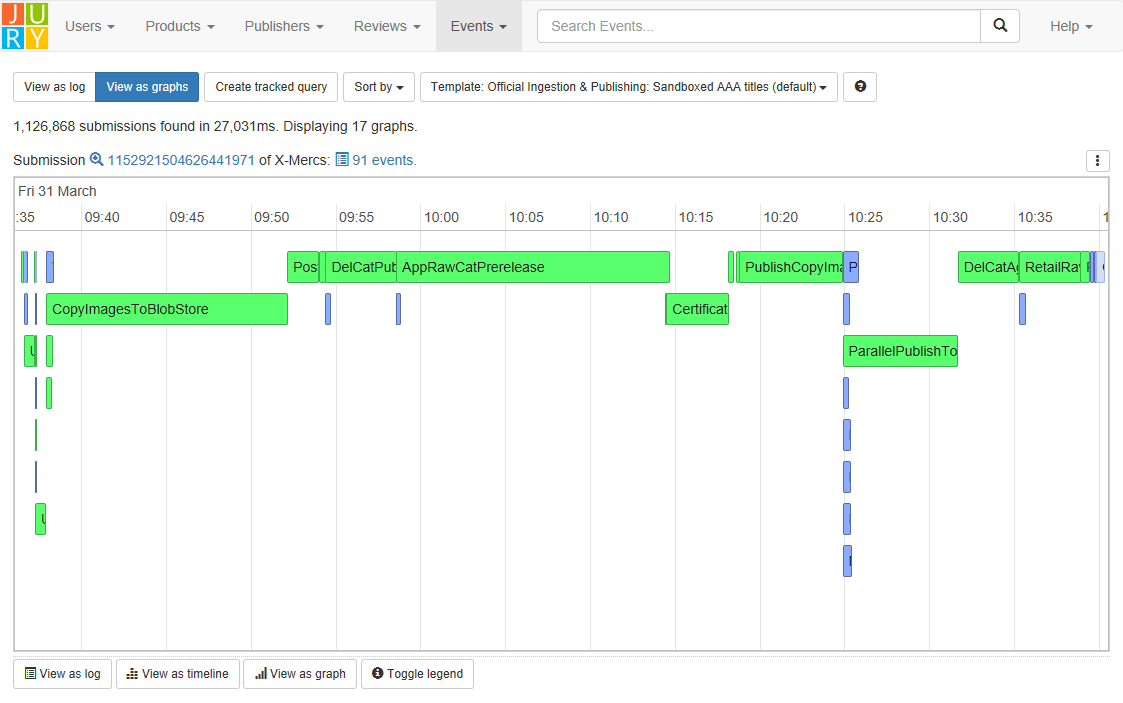
\includegraphics[width=\linewidth]{gfx/screenshots/timeline.png}
\caption{Timeline view \label{fig:timeline}}
\end{figure}

Each trace returned by the query is visualized as a timeline or a graph. On top of the visualization the user can see the basic information about the trace containing the submission ID and the name of the product.
Under the visualization there are options to choose how the visualization is displayed (between the log view, the graph view, and the timeline view) and an option to toggle help.
The visualization can be manipulated with the mouse or a touch screen. It allows panning and zooming actions.
The user can select or mouseover individual events to see all the metadata related to the event.

In the timeline view (Figure \ref{fig:timeline}), the visualization is set on top of a horizontal axis that corresponds to time. The activities shown have start and end times which can be seen visually or in the metadata.
Parallel activities are stacked on top of each other.
Figure \ref{fig:estimates} shows the estimations for an incomplete submission.
The activities yet to happen are drawn with a faint blue color and their estimated start and end times are visualized similarly as the logged activities.
The red line displays the current time.
The user can visually see the status of the submission and the activities that are predicted to have happened already.

\begin{figure}[htb]
\centering 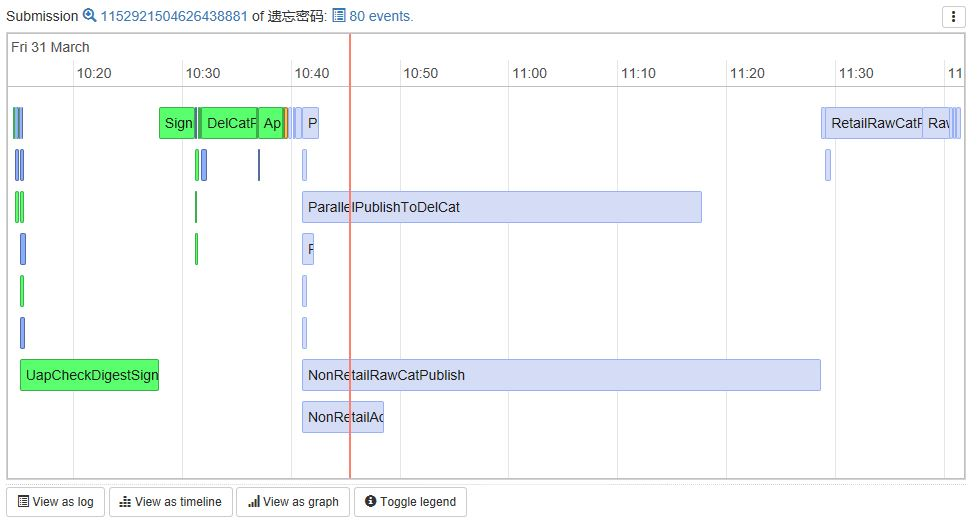
\includegraphics[width=\linewidth]{gfx/screenshots/estimates.jpg}
\caption{Timeline view with estimates \label{fig:estimates}}
\end{figure}

Figure \ref{fig:graph} shows the alternate directed graph view. In the graph view the directed graph is drawn for the user. The graph nodes are interactive and the edges act as two-dimensional springs.
The user can thus manipulate and move the nodes. Panning and zooming actions are also enabled.

\begin{figure}[htb]
\centering 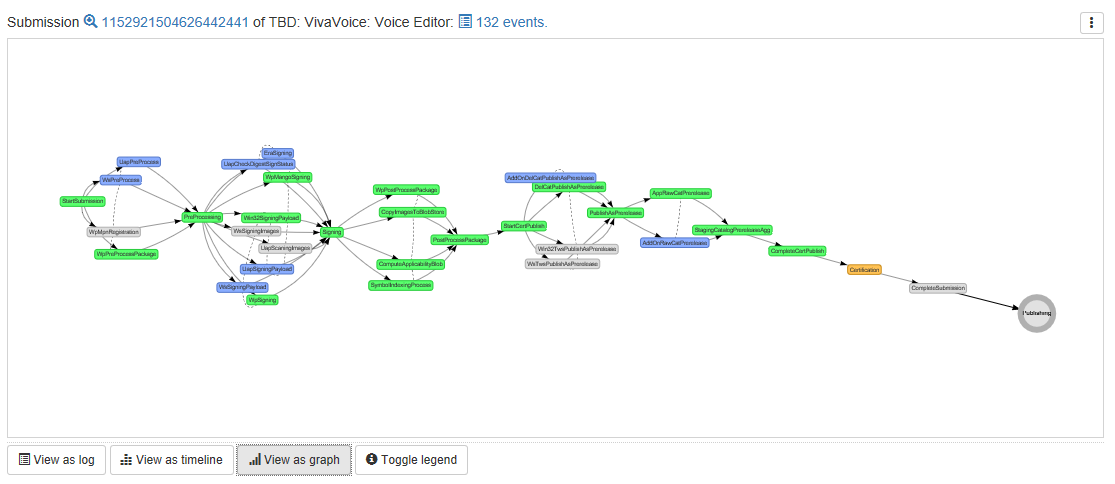
\includegraphics[width=\linewidth]{gfx/screenshots/graph.png}
\caption{Graph view \label{fig:graph}}
\end{figure}

In the user meetings in between the two iterations, the timeline view was unanimously agreed to be the more useful visualization. 
The graph view was seen as ``unnecessarily complex'' and the physics animation was perceived as ``annoying'' and ``fidgety''. 
In other words, the graph view didn't offer a clear ``big picture'' since it required the user to manipulate the view before it showed the information clearly. 
The users wanted the graph view to have more organization, and several users asked for automated sorting or positioning of the graph nodes.

Conversely, the static and clear positioning of the timeline view was seen as useful.
Since the view was pre-generated and organized on a static timeline, most graphs would end up looking exactly the same without any manipulation.
A user would be able to visually scan the list of graphs and notice anything significantly different.
The user could then investigate the distinct graph to find out whether the difference is a result of a failure.
The users commented that they did not even need to pay attention to the specific nodes but only focus on the overall shape of the graph.

To evaluate the results of the machine learning models, I first calculated a baseline for comparison.
The baseline consists of the same simple statistics as were used for the estimates in the application, the TP50 (median) and the TP75.
I calculated these two values for each transition (graph edge) based on the training set to construct a simple model. 
In the model each transition corresponds to a single value (the TP50 or the TP75). 
When predicting, the model always returns this value based on the transition in question.
Table \ref{tab:statresults} lists the results from this baseline model for both training datasets described in section \ref{sec:ml-estimation}. 
The values of \textit{mean absolute error} and \textit{root mean square error} are listed.

\begin{table}[htb]
\begin{center}
\begin{tabularx}{\linewidth}{| X | r | r |}
\hline
Dataset + Model & Mean Absolute Error & RMSE \\
\hline
\textbf{JSON template} &  & \\
TP50 value (median)         & 573.3 & 5871.4 \\
TP75 value                  & 710.5 & 5484.2 \\
\hline
\textbf{Automatically generated template} &  & \\
TP50 value (median)         & 919.6 & 9937.3 \\
TP75 value                  & 954.0 & 9904.8 \\
\hline
\end{tabularx}
\end{center}
\caption{Results from plain statistics}
\label{tab:statresults}
\end{table}

I used the same training and testing sets to find the same error values for each machine learning model.
The parameters used for the models are listed in table \ref{tab:modelparameters}.
The model parameters correspond to the parameters listed in the documentation \cite{azurebdt,azurepoisson}.
The error values are listed in table \ref{tab:mlresults}.
The first two columns list the error values for the boosted decision trees model (BDT).
Again, the values of mean absolute error (``Absolute'') and root mean square error (``RMSE'') are listed.
The same models are used for both datasets.

\begin{table}[htb]
\begin{center}
\begin{tabular}{| l  r | l  r |}
\hline
\multicolumn{2}{|c|}{Boosted Decision Trees} & \multicolumn{2}{|c|}{Poisson Regression} \\
\hline
Mode & Single         & Mode & Single \\
Number of leaves & 20   & Optimization tolerance & 1E-07 \\
Number of samples & 10  & L1 regularization weight & 1.0 \\
Learning rate & 0.2             & L2 regularization weight & 1.0 \\
Total number of trees & 100     & Memory size for L-BFGS & 20 \\
\hline
\end{tabular}
\end{center}
\caption{Model parameters from ML testing}
\label{tab:modelparameters}
\end{table}

I calculated the error values for all the different sets of features, as described in section \ref{sec:featureset}.
The first model was generated by only using the features available in the application package.
The second model uses the current time in seconds since the submission start as an additional feature.
The next two models use the new features I created for resubmissions and entering a manual review.
I also used both these two features together to test the models, and lastly all these three features combined.

\begin{table}[htb]
\begin{center}
\begin{tabularx}{\linewidth}{| X | r | r | r | r |}
\hline
~ & \multicolumn{2}{c|}{BDT} & \multicolumn{2}{c|}{Poisson} \\
Dataset + Model & Absolute & RMSE & Absolute & RMSE \\
\hline
\textbf{JSON template} &  &  &  &  \\
No extra features                   & 809.1 & 6290.7 & 881.1 & 5970.6 \\
with current time                   & 825.2 & 6130.3 & 881.1 & 5971.0 \\
with manual review                  & 689.7 & 5819.0 & 809.3 & 5800.9 \\
with resubmission                   & 831.5 & 6255.3 & 881.1 & 5971.2 \\
with manual review and resubmission & 703.7 & 5807.5 & 808.9 & 5800.8 \\
with all extra features             & 693.5 & 5801.9 & 808.3 & 5800.4 \\
\hline
\textbf{Automatically generated template} &  &  &  &  \\
No extra features                   & 994.8 & 5756.3 & 1243.9 & 6563.3 \\
with current time                   & 1099.7 & 6470.5 & 1225.8 & 6558.7 \\
with manual review                  & 815.1 & 5332.1 & 1038.5 & 5785.0 \\
with resubmission                   & 1004.3 & 5845.3 & 1219.1 & 6553.8 \\
with manual review and resubmission & 806.5 & 5428.4 & 1038.4 & 5785.7 \\
with all extra features             & 787.8 & 5234.4 & 1038.6 & 5785.4 \\
\hline
\end{tabularx}
\end{center}
\caption{Results from the best ML models}
\label{tab:mlresults}
\end{table}

% \subsection{Evaluation}
% \label{sec:evaluation}

\clearpage
\section{Conclusion}
\label{sec:conclusion}

% % Tutkimustuloksien merkityst\"a on aina syyt\"a arvioida ja tarkastella
% % kriittisesti.  Joskus tarkastelu voi olla t\"ass\"a osassa, mutta se
% % voidaan my\"os j\"att\"a\"a viimeiseen osaan, jolloin viimeisen osan nimeksi
% % tulee >>Tarkastelu>>. Tutkimustulosten merkityst\"a voi arvioida my\"os
% % >>Johtop\"a\"at\"okset>>-otsikon alla viimeisess\"a osassa. 

% % T\"ass\"a osassa on syyt\"a my\"os arvioida tutkimustulosten luotettavuutta.
% % Jos tutkimustulosten merkityst\"a arvioidaan >>Tarkastelu>>-osassa,
% % voi luotettavuuden arviointi olla my\"os siell\"a. 

%\item How can a real-time event log from multiple sources and multiple concurrent workflows be dynamically transformed into a model that describes the process? 
%\nyi{Talk about success with graph generation}\\

The goal of this thesis was to find out whether past event logs could be used to detect anomalies in real-time. 
The first research question asked how event log data can be used to generate a model that describes the process.
In this thesis I explored the options of using WF-nets and directed graphs to model processes.
The directed graphs were chosen to be satisfactory for modeling the workflows in the Microsoft Store.
The models were visualized as both directed graphs and on a horizontal timeline.
The users found the static and pre-arranged timeline view to be useful. 
However, the graph view was deemed to be useful for debugging the process, since it shows the relationships and dependencies between the activities.
For this reason I kept both views as options for the user to choose from.

%\nyi{Finding bugs in system (race conditions!) based on graphs}\\
The models were evaluated by comparing them to the official workflow descriptions that were used by engineers to maintain the models. 
With a short time span of events the models were noisy and lacked some of the parallelism that the real processes had.
However, with event logs longer than three days the models captured all the activities and their dependencies.
In one instance the graph showed incorrect dependencies which proved to be a race condition bug in the actual system that caused the process workflow to execute in an invalid order.
The results from the discovered model were used to fix the race condition in the store system.

%\nyi{Changes in the system reflected real time (also a strength?)}\\
The model was always generated from the past three days or seven days of data, based on the query. Because of this, any changes to the workflows started to appear in the models within this time window. 
The changes were automatically picked up by the process discovery algorithm and required no engineer interaction.

%\item How can the model and past log data be used to predict future events and their times?
The second research question asked how the model could be used to predict future events and their times. 
The predictions I ended up using in the thesis were based on simple statistics. 
The statistical approach was deemed to be sufficient for the use case of predicting activities. 
Since many of the activities are fairly short, small variations in the predictions are acceptable. 
In addition, an overestimation is always a better result in this use case.
For example, if an event is estimated to arrive in five minutes and it arrives in four, the user is happy.
Since the system has a lot of variation in activity durations even when the system is functioning normally, detecting small anomalies is not useful to the user and can even be seen as noise.

Machine learning was considered an option to improve the predictions. The idea was that the variation in delay would depend on the characteristics of the submission such as the file size.
However, the machine learning models did not significantly improve the results of the predictions.
When comparing the results for the simple statistical model using the median and the TP75 values (figure \ref{tab:statresults}) and the results from the machine learning models (figure \ref{tab:mlresults}) there is no significant difference.
With the first data set (``JSON template'') the machine learning models did not even reach the error values of the statistical approach.
With the second data set (``Automatically generated template'') the machine learning model showed a slight improvement over the statistical model.
However, since most of the activities have lengths of less than five minutes, an average prediction error of more than 10 minutes is still not a good prediction.
Since slightly overestimating an ETA was seen as acceptable by the users, the complexity and engineering work required to implement the machine learning models in production was not seen as necessary.
A simple statistical implementation with simpler code was seen as more worthwhile than a possible slight increase in prediction accuracy.

%\nyi{Talk about negatives with machine learning models}\\
%\nyi{Reason why they didn't end up working}

The reasons why the machine learning models did not provide useful results can be explored.
Since both models (Poisson regression and boosted decision trees) reached similar results even though they function very differently, it suggests that the data sets were too noisy or the results did not depend enough on the used features.
Even after I identified the two possible features that could be added to the data sets (the manual review feature and the resubmission feature), it did not significantly improve the results.
The result from my exploration was that other features such as time of day, system congestion and network status was affecting the times more than the characteristics of the application package itself.

In conclusion, the users agreed that the statistical estimations were useful in the visualizations, since they allow the user to visually see what part of the workflow the submission is in.
Furthermore, the predictions give the user a simple estimate for the completion time. 
For many users, the exact time is not important, but knowing whether the estimation is in the order of minutes or hours was seen as significant.

%\item How can the predictions be used to detect anomalies in new events (or lack thereof)?

The third and final research question asked if the predictions could be used to automatically notify the users about anomalies without the need for the user to look at the visualizations.
The main use case was to detect submissions that are ``stuck''.
The expression ``stuck'' meant a submission that has stayed in a particular activity for an abnormally long period of time, usually because of an error in the submission data or in the activity processor.
This means that the system should send a notification to a relevant user about any significant anomalies, whereas small anomalies are not important.
The notification system described in section \ref{sec:notifications} was proven to function correctly after the initial testing. 
However, since the number of stuck submissions is very small compared to the massive amount of submissions in the store, accurate evaluation was difficult to make during my short evaluation period.

The project was released into the production systems and has been in use in Jury.
At the time of this writing (July 2017), in the past 90 days 232 unique users have used the events-section of Jury, and of those users 157 have used the workflow visualizations.
Only seven users currently use the automatic email notification features.

%%%%%%%%%%%%%%%%%%%%%%%%%%%%%%%%%%%%%%%%%%%%%%%%%%%%%%%%%%%%%%%%%%%%%%%%%%%%%%%%

\subsection{Benefits} 
\label{sec:benefits}

This thesis research achieved its main goal, which was to create visualizations for the internal Microsoft users to help maintain and monitor the store systems and submissions.
The system was released into production immediately and all the users using Jury are now able to use the events, visualizations, and the notification system.

More than 150 users have used the notifications within the past three months which I consider significant, 
since the users of Jury are all internal and most of them are users from a few specific teams within the company.
The notification system needs to be publicized within the company more, since it seems that most users are not aware it exists.

The accuracy of the models and the real-time overlay functionality was praised by the users and is seen as a success.
Most studies I referenced in this thesis focus on analyzing past logs to find useful information.
My thesis work had a significant focus on the real-time functionality and the ability to dynamically adapt to the events as they arrive.
I was able to successfully use the events and leverage the process models in a real-time scenario.

\subsection{Limitations and Future work}

Further research should be made into the process discovery algorithm options.
This study only focused on the \textalpha-algorithm and its applications. 
Different graph generation algorithms such as transition systems \cite{van2013discovering} should be explored and tested in this particular application.

The current system's prediction accuracy is acceptable but not particularly accurate.
For accurate predictions and better machine learning possibilities more research is needed on the aspects of the store which affect the activity processing times.

Furthermore, the real-time aspect of process mining is something that needs further examination. In this thesis I adapted existing methods designed for analyzing past event logs to be used in a real-time scenario.
Further research should be made to specifically examine the challenges and possibilities of real-time events.



%%%%%%%%%%%%%%%%%%%%%%%%%%%%%%%%%%%%%%%%%%%%%%%%%%%%%%%%%%%%%%%%%%%%%%%%%%%%%%%%
%%%%%%%%%%%%%%%%%%%%%%%%%%%%%%%%%%%%%%%%%%%%%%%%%%%%%%%%%%%%%%%%%%%%%%%%%%%%%%%%
%%% End
%%%%%%%%%%%%%%%%%%%%%%%%%%%%%%%%%%%%%%%%%%%%%%%%%%%%%%%%%%%%%%%%%%%%%%%%%%%%%%%%
%%%%%%%%%%%%%%%%%%%%%%%%%%%%%%%%%%%%%%%%%%%%%%%%%%%%%%%%%%%%%%%%%%%%%%%%%%%%%%%%

\clearpage
%% The \phantomsection command is necessary for hyperref to jump to the 
%% correct page, in other words it puts a hyper marker on the page.

\phantomsection
\addcontentsline{toc}{section}{References}

\printbibliography

%% Appendices
%\clearpage
%\thesisappendix

\end{document}
